\newpage
\appendix
\section{Transformer with Hyper-Connections}
\label{app:trans_with_hc}
\begin{figure}[h]
    \begin{center}
    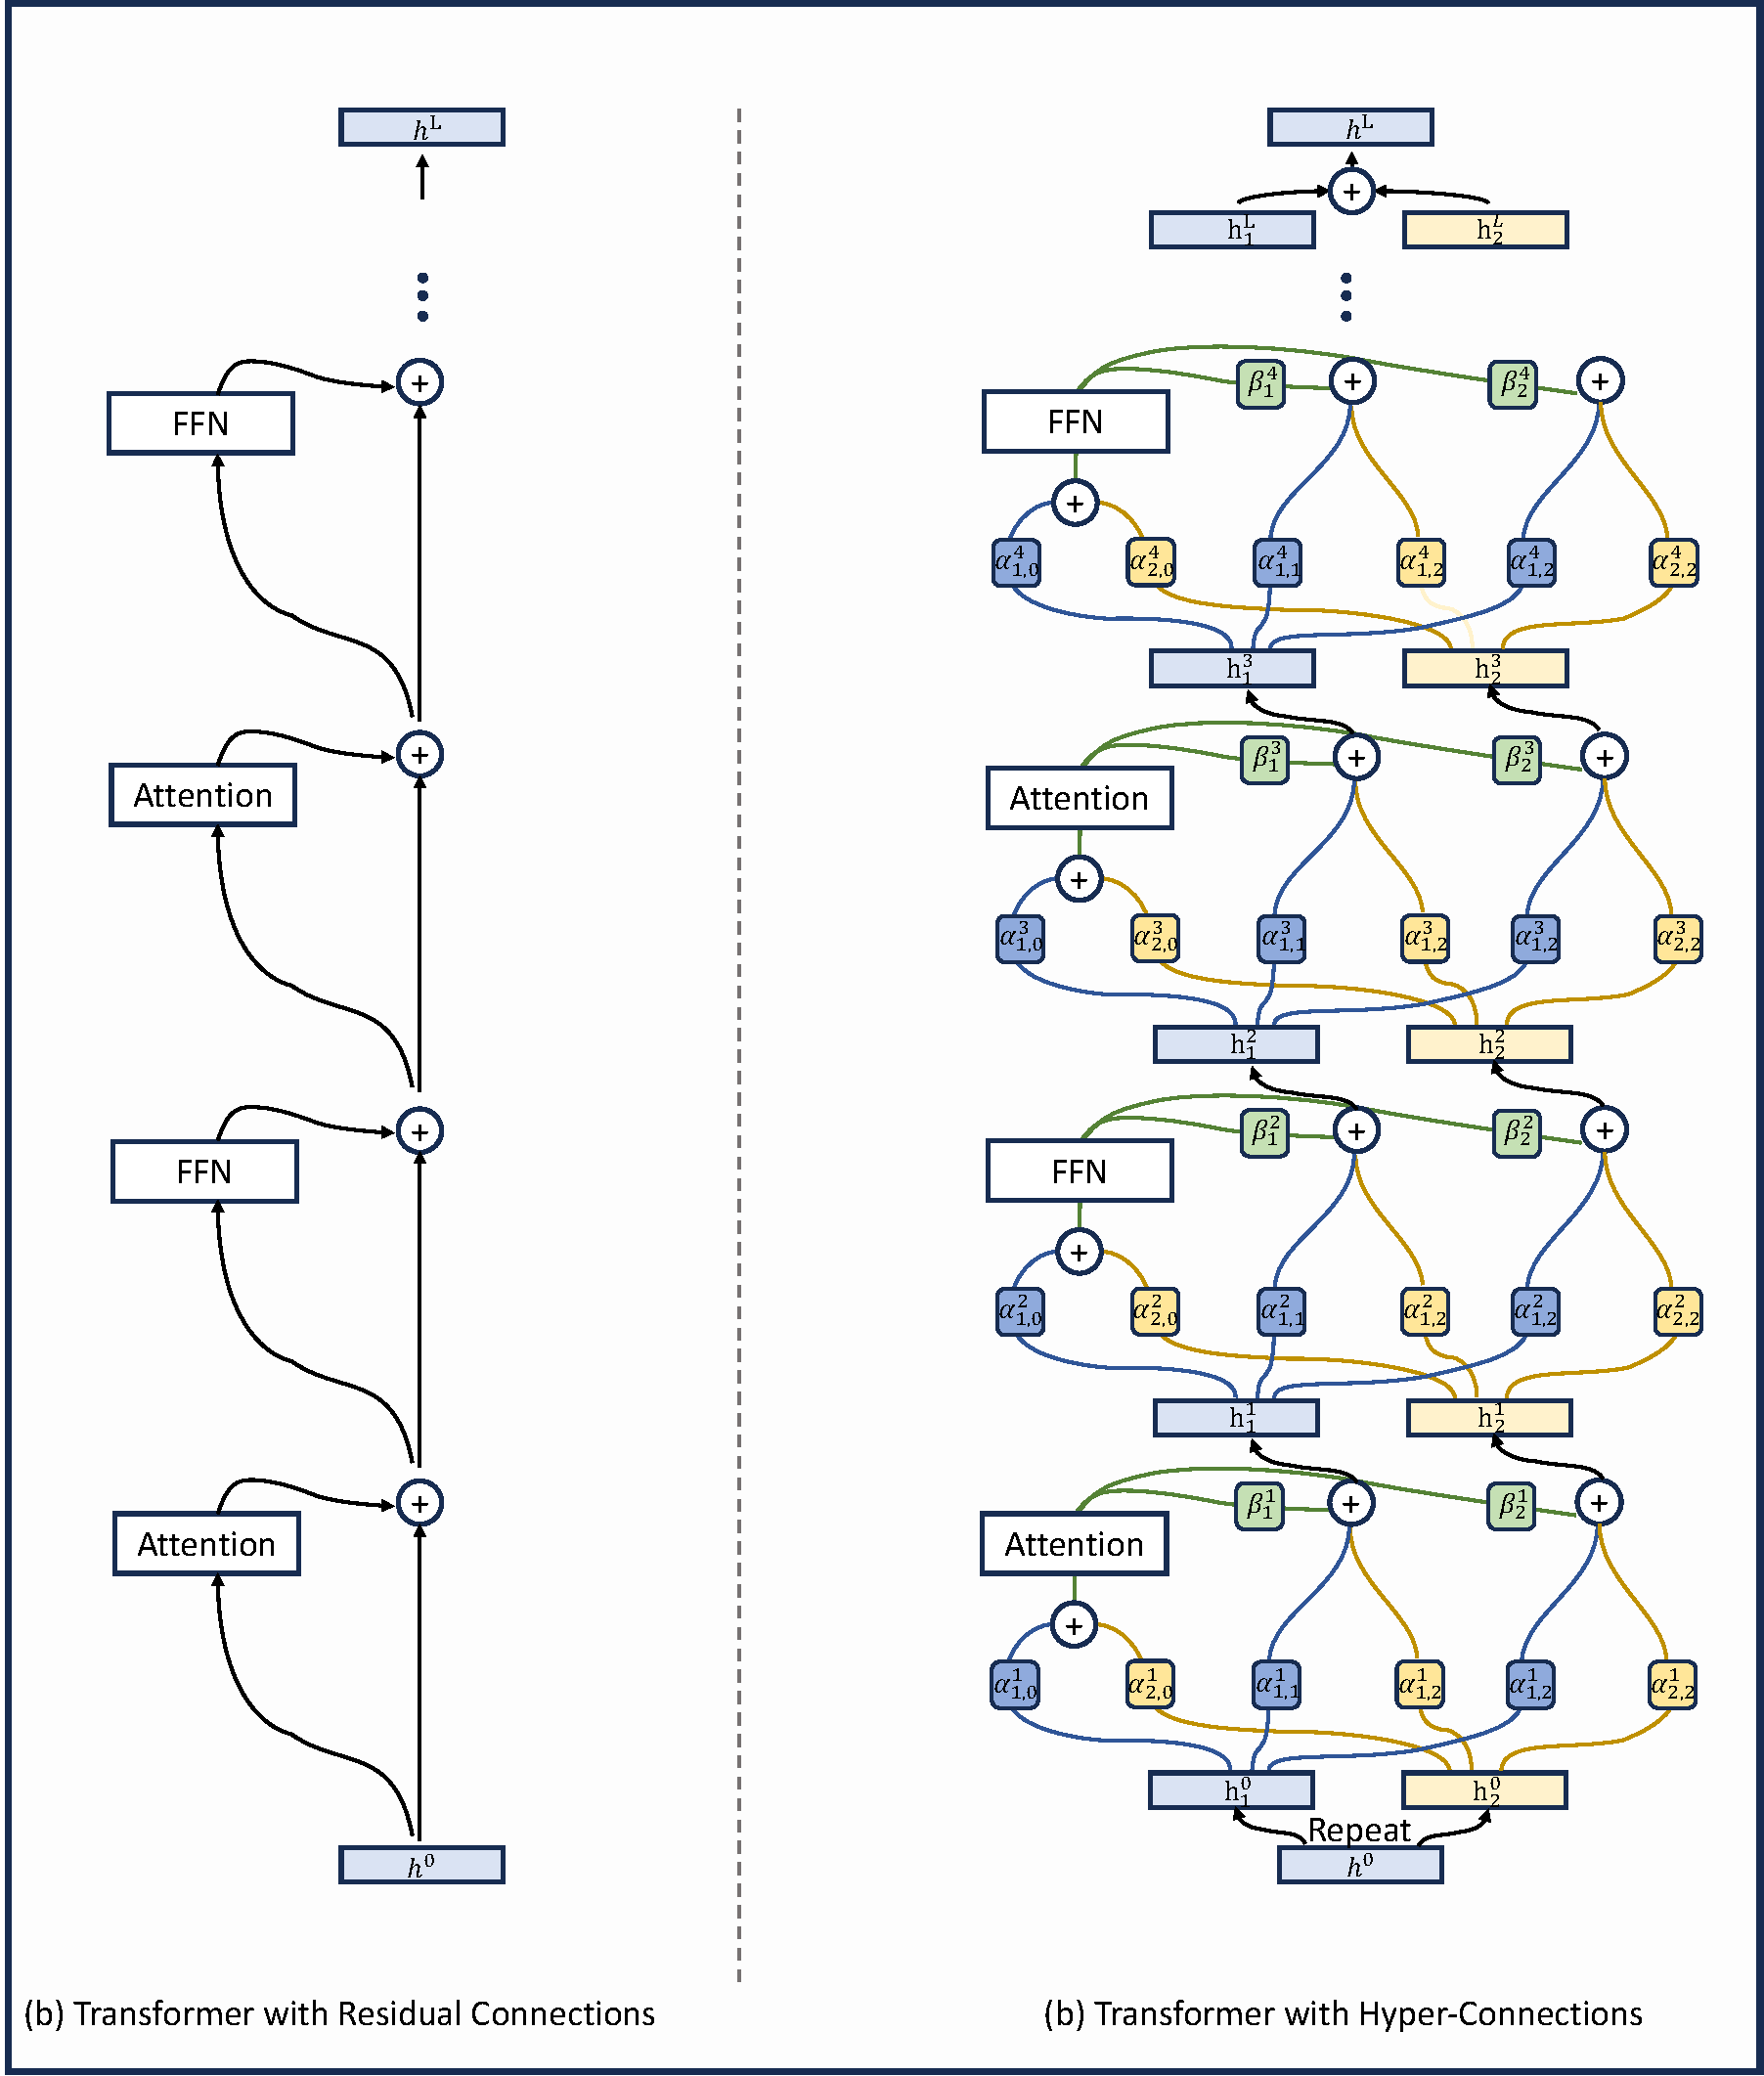
\includegraphics[width=1\textwidth]{fig/trans_with_hc.pdf}
    \end{center}
  \caption{\newtext{Comparison between transformers with hyper-connections and that with residual connections.}}
    \label{fig:trans_with_hc}
\end{figure}

\newpage

\section{\newtext{Parameters, Computation and Memory Footprint Analysis}}
\label{app:para_comp_mem_analysis}
\newtext{{\bf Static Hyper-Connections.} All learnable parameters are included in the hyper-connection matrix $\mathcal{HC}$ in Eq.~\ref{eq:shc}. The number of parameters in one $\mathcal{HC}$ is given by:
\begin{equation}
    \left|\theta_{\texttt{SHC}}\right|= |\theta_{\mathbf{B}}| + |\theta_{\mathbf{A}}|= n + n \cdot (n+1)=n \cdot (n+2),
\end{equation}
where $n$ is the expansion rate, $|\theta_{\mathbf{B}}|$ is the number of parameters in $\mathbf{B}$ in $\texttt{SHC}$, and $|\theta_{\mathbf{A}}|$ is the number of parameters in $\mathbf{A}$. Each layer contains two hyper-connection modules (one for the self attention and one for the feedforward network). Thus, the number of extra parameters is:
\begin{equation}
P_{\texttt{extra}}=\left|\theta_{\texttt{SHC}}\right| \times 2 \times L,
\end{equation}
where $L$ is the number of layers. For example, in \texttt{OLMo-1B-SHC$\times$4}, $P_{\texttt{extra}}=4\times (4+2) \times 2 \times 16=768$.}

\newtext{{\bf Dynamic Hyper-Connections.} The parameters of DHC are defined in Eqs.~\ref{eq:norm}, \ref{eq:B}, \ref{eq:Am}, and \ref{eq:Ar}, and the number of parameters is given by:
\begin{align}
    \left|\theta_{\texttt{DHC}}\right| &= |\theta_{\texttt{norm}}| + |s_{\beta}| + |\theta_{\mathbf{W}_\beta}| + |\theta_{\mathbf{B}}| + 
    |s_{\alpha}| + |\theta_{\mathbf{W}_m}| + |\theta_{\mathbf{A}_m}| +
    |\theta_{\mathbf{W}_r}| + |\theta_{\mathbf{A}_r}| \\
    &= |\theta_{\texttt{norm}}| + 1 + d_{\texttt{model}} + n + 1 + d_{\texttt{model}} + n + d_{\texttt{model}}\times n + n\times n \\
    &=|\theta_{\texttt{norm}}| + d_{\texttt{model}}\times (n+2)  + n \times (n+2) + 2,
\end{align}
where $d_{\texttt{model}}$ is the dimension of the hidden states in the transformer, and $|\theta_{\texttt{norm}}|$ depends on the type of normalization module. In OLMo models, there are no parameters for normalization, so $|\theta_{\texttt{norm}}|=0$. In OLMoE, $|\theta_{\texttt{norm}}|=d_{\texttt{model}}$. Similar to the static hyper-connections, the number of extra parameters is:
\begin{equation}
P_{\texttt{extra}}=\left|\theta_{\texttt{DHC}}\right| \times 2 \times L,
\end{equation}
For example, for \texttt{OLMo-1B-DHC$\times$4}, $P_{\texttt{extra}}=(0 + 2048\times (4+2)  + 4 \times (4+2) + 2)\times 2 \times 16=394,048$.}

\newtext{The number of parameters for \texttt{DHC} and \texttt{SHC} used in the experiments is detailed in Table~\ref{tab:params_comparison}, while their corresponding FLOPs comparisons are provided in Table~\ref{tab:flops_comparison}. Regardless of whether \texttt{SHC} or \texttt{DHC} is used, the additional parameters and computational overhead introduced are minimal and can be considered negligible.}

\begin{table}[h]
\centering
\caption{Comparison of number of parameters.}
\begin{tabular}{lccc}
\toprule
\textbf{Method}       & \makecell{\textbf{HC Params(B)}} & \makecell{\textbf{Total Params(B)}} & \makecell{\textbf{Total Params $\Delta$ rate (\%)}} \\ 
\midrule
OLMo-1B             & -                   & 1.17676442  & - \\ 
OLMo-1B-SHC$\times$2       & 0.0000026           & 1.17676467  & \bf{+0.00002\%} \\ 
OLMo-1B-SHC$\times$4       & 0.0000077           & 1.17676518  & \bf{+0.00007\%} \\ 
OLMo-1B-DHC$\times$2       & 0.0002625           & 1.17702688  & \bf{+0.02230\%} \\ 
OLMo-1B-DHC$\times$4       & 0.0003940           & 1.17715846  & \bf{+0.03349\%} \\ 
\midrule  % Add a thicker line between 1B and 7B
OLMo-7B             & -                     & 6.88809574  & - \\ 
OLMo-7B-DHC$\times$4       & 0.0013124            & 6.88967027  & \bf{+0.02286\%} \\ 
\midrule  % Add a thicker line between 1B and 7B
OLMoE-1B-7B         & -                     & 6.91909427  & - \\ 
OLMoE-1B-7B-DHC$\times$4   & 0.0003940            & 6.91948832  & \bf{+0.00570\%} \\ 
\bottomrule
\end{tabular}
\label{tab:params_comparison}
\end{table}

\newtext{{\bf Computation Analysis.} 
The main computational cost of SHC and DHC lies in line 5 of Algorithm~\ref{alg:hyper_connections}, where the complexity is $\mathcal{O}(d_{\text{model}} \times n \times (n+1))$. The computational cost of the FFN is $\mathcal{O}(2 \times d_{\text{model}} \times d_{\text{ffn}})$, and that of the projection part of attention is $\mathcal{O}(4 \times d_{\text{model}} \times d_{\text{model}})$. Since $\mathcal{O}(d_{\text{model}} \times n \times (n+1)) \ll \mathcal{O}(4 \times d_{\text{model}} \times d_{\text{model}}) < \mathcal{O}(2 \times d_{\text{model}} \times d_{\text{ffn}})$, the computational cost of HC is negligible compared to the cost of both FFN and the attention projection part. Here, $d_{\text{ffn}}$ is the inner dimension of the FFN. The detailed computation cost statistics are presented in Table~\ref{tab:flops_comparison}.}

\newpage
\begin{table}[h]
\centering
\caption{FLOPs per token in forward pass.}
\begin{tabular}{lccc}
\toprule
\textbf{Method}       & \makecell{\textbf{HC FLOPs (G)}} & \makecell{\textbf{Total FLOPs (G)}} & \makecell{\textbf{Total FLOPs $\Delta$ rate (\%)}} \\ 
\midrule
OLMo-1B               & -              & 2.3536  & - \\ 
OLMo-1B-SHC$\times$2         & 0.0010         & 2.3545  & \textbf{+0.038\%} \\ 
OLMo-1B-SHC$\times$4         & 0.0031         & 2.3566  & \textbf{+0.127\%} \\ 
OLMo-1B-DHC$\times$2         & 0.0020         & 2.3554  & \textbf{+0.076\%} \\ 
OLMo-1B-DHC$\times$4         & 0.0049         & 2.3583  & \textbf{+0.200\%} \\ 
\midrule
OLMo-7B           & -              & 13.3647  & - \\ 
OLMo-7B-DHC$\times$4     & 0.0197         & 13.3844  & \textbf{+0.147\%} \\ 
\midrule
OLMoE-1B-7B           & -              & 2.3580  & - \\ 
OLMoE-1B-7B-DHC$\times$4     & 0.0049   & 2.3629  & \textbf{+0.208\%} \\ 
\bottomrule
\end{tabular}
\label{tab:flops_comparison}
\end{table}

\newtext{{\bf Memory Footprint.} The introduction of HC results in a minor increase in activation memory usage during training. For a transformer model with $L$ layers, a model dimension of $d_{\text{model}}$, batch size $b$, sequence length $s$, and number of attention heads $a$, the activation memory is calculated as $sbd_{\text{model}}L(34 + 5as/d_{\text{model}})$, as outlined in \cite{korthikanti2022reducing}. Incorporating HC with an expansion rate of $n$ adds an extra memory overhead of $2nsbd_{\text{model}}L$. For $n=2$, this contributes less than $15\%$ to the total memory usage of a standard transformer. Notably, the memory consumption is mostly driven by the weight parameters, which experience only a slight increase with HC. Additionally, given HC's low computational cost, the hidden states generated by HC can be discarded post forward pass and recomputed during backpropagation to further optimize memory usage. With this approach, the additional memory requirement is reduced to $nsbd_{\text{model}}$. 
During inference, the memory usage for activations is largely determined by the Key-Value cache, which is not impacted by the extra activations brought by HC. Moreover, the hidden states from earlier layers can be released as soon as the next layer's computations start, significantly lowering memory requirements.}

\newpage
\section{MoE 1B/7B Model Experiments}
\begin{figure}[h]
    \begin{center}
    \includegraphics[width=0.9\textwidth]{fig/OLMoE_1B7B.pdf}
    \end{center}
  \caption{Loss curves in V3 validation sets and accuracy curves on downstream tasks for \texttt{OLMoE-1B7B} and \texttt{OLMoE-1B7B-DHC$\times{4}$} models.}
    \label{fig:moe_1b7b_full_results}
\end{figure}

\newpage
\section{7B Model Experiments}
\begin{figure}[h]
    \begin{center}
    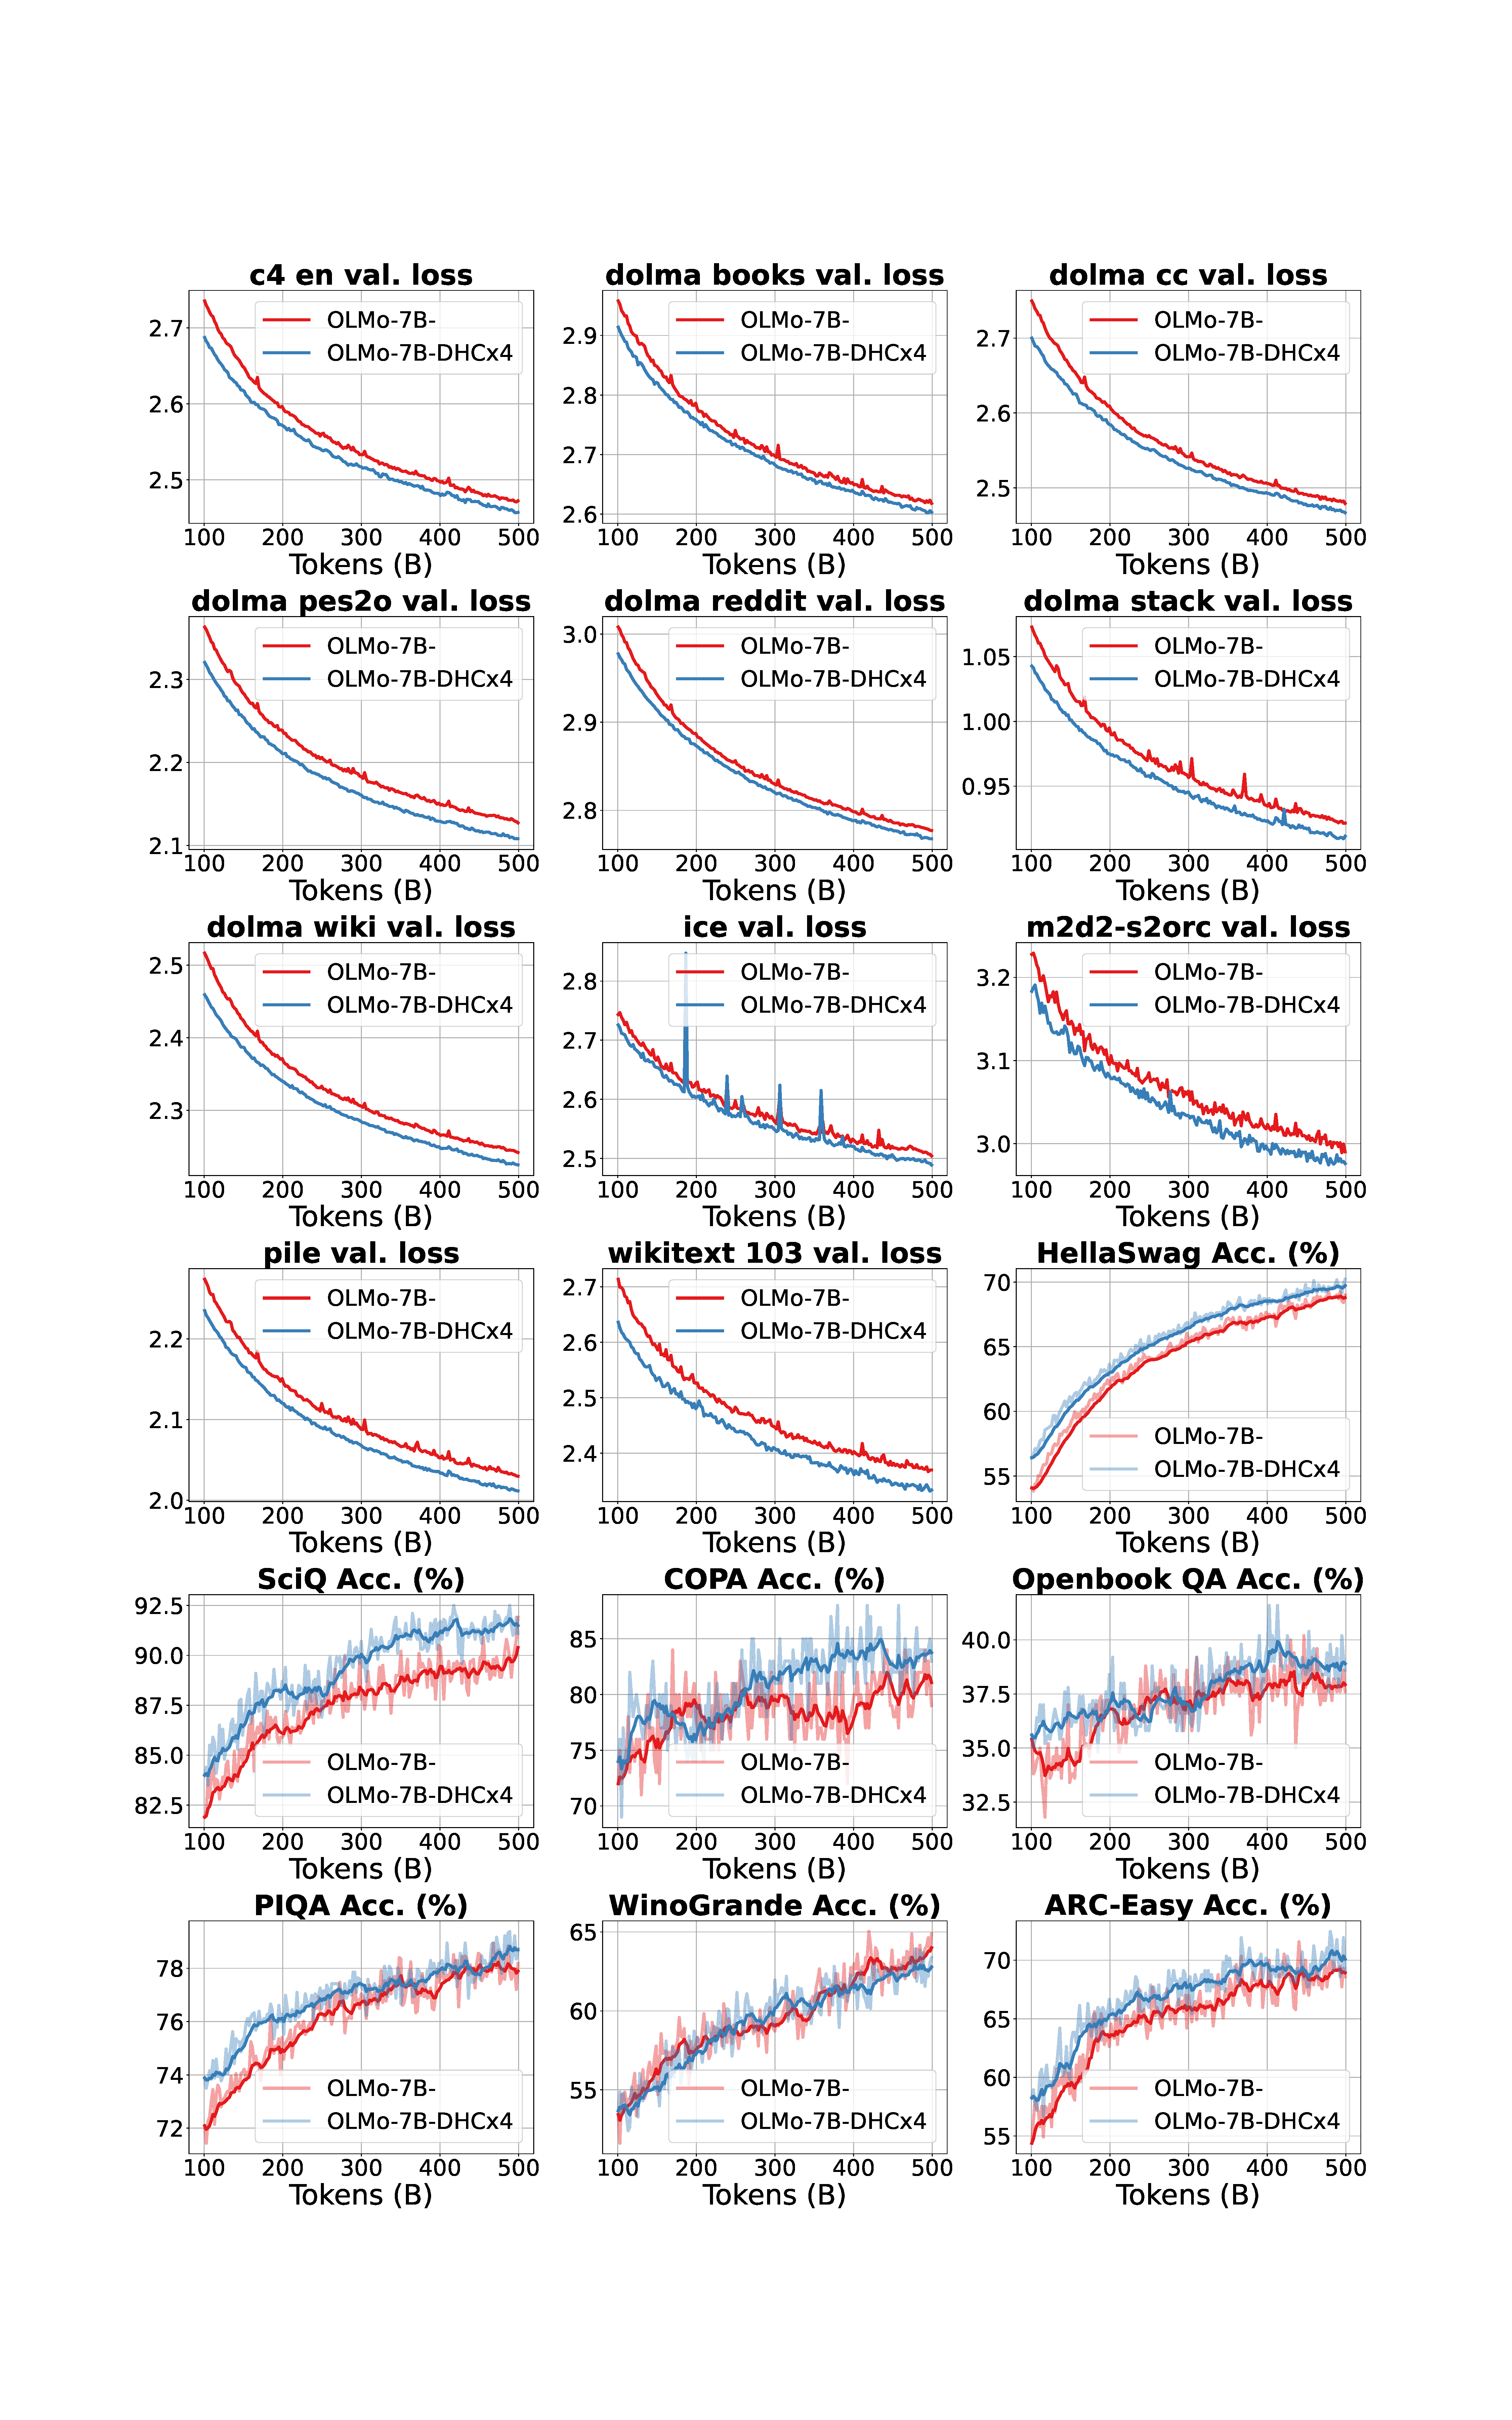
\includegraphics[width=0.82\textwidth]{fig/7B_v3_downstream.pdf}
    \end{center}
  \caption{Loss curves in V3 validation set and accuracy curves on downstream tasks for \texttt{OLMo-7B} and \texttt{OLMo-7B-DHC$\times$4} models.}
    \label{fig:7b_full_results}
\end{figure}

\newpage
\section{Vision Experiments}
\label{sec:vision_exp}
\textbf{Datasets.} We use the ILSVRC-2012 ImageNet dataset~\citep{deng2009imagenet} with 1k classes and 1.3M images (see ImageNet in the following) for image generation and classification. 
\subsection{Image Generation}
To investigate the generalizability of hyper-connections in image generation, our experiments are conducted using the DiT framework~\citep{Peebles2022DiT} training the models for 1400 epochs. In order to save experimental costs, we use FP16 precision, introduce flash-attention to speed up training, and introduce QK-Norm~\citep{wortsman2023small} to stabilize training.


\begin{table}[h]
\centering
\caption{Benchmarking class-conditional image generation on ImageNet 256$\times$256, with cfg=1.50. \textbf{NP}, \textbf{P}, and \textbf{R} are short for Numerical Precision, Precision, and Recall, respectively.}
\begin{tabular}{lcccccccc}
\toprule
\textbf{Method} & \textbf{NP} & \textbf{QK-Norm} & \textbf{Size (M)} & \textbf{FID$\downarrow$} & \textbf{sFID$\downarrow$} & \textbf{IS$\uparrow$} & \textbf{P$\uparrow$} & \textbf{R$\uparrow$} \\
\midrule
\cellcolor{gray!20}DiT-XL/2 & \cellcolor{gray!20}\texttt{FP32} & \cellcolor{gray!20}\ding{55} & \cellcolor{gray!20}675 & \cellcolor{gray!20}2.27 & \cellcolor{gray!20}4.60 & \cellcolor{gray!20}278.24 & \cellcolor{gray!20}0.83 & \cellcolor{gray!20}0.57 \\
\midrule
DiT-XL/2 & \texttt{FP16} & \ding{51} & 675 & 2.36 & 4.54 & 269.46 & 0.83 & 0.58 \\
DiT-1B/2 & \texttt{FP16} & \ding{51} & 983 & 2.13 & 4.50 & 288.69 & 0.82 & 0.59 \\
\midrule
DiT-XL/2-SHC$\times$2 & \texttt{FP16} & \ding{51} & 675 & 2.18 & 4.52 & 287.24 & 0.82 & 0.60 \\
\bottomrule
\end{tabular}
\label{tab:imagenet}
\end{table}

Our experimental results demonstrate that DiT models incorporating hyper-connections exhibit comparable performance metrics to DiT models with 50\% more parameters. This finding underscores the efficiency and efficacy of hyper-connections in enhancing model performance without increasing model size.


\subsection{Image Classification}
For the image classification experiments, we train ViT/16-Base and ViT/16-Large models with images at a resolution of $224 \times 224$ for 300 epochs, following the experimental setup used by \citep{dosovitskiy2020image}.To speed up the training process, we use bfloat16 numerical precision. The training configuration is detailed in Table \ref{tab:vit_hyperparameters}. Within this configuration, we replace the residual connections with static and dynamic hyper-connections, referred to as SHC and DHC, respectively, using an expansion rate of $n=2$. The top-1 accuracy results are presented in Table \ref{tab:vit_comparison}, and the training loss curves for ViT/16-Large and ViT/16-Large with DHC$\times$2 are shown in Fig.~\ref{fig:vit_loss}.

For the Base model (85M), our re-implemented ViT/16 achieves 76.38\% accuracy on $224 \times 224$ images. The SHC and DHC enhance performance to 77.60\% and 77.26\%, respectively. representing relative increases of \textbf{1.22\%} and \textbf{0.88\%}. For the Large model (307M parameters), ViT/16 achieves 77.25\% accuracy. The SHC and DHC configurations further enhance accuracy to 78.38\% and 79.94\%, respectively. This corresponds to relative improvements of \textbf{1.13\%} and \textbf{2.69\%}, with DHC showing the highest performance. These results demonstrate that hyper-connections (SHC and DHC) significantly improve accuracy, especially in the Large model scale.

\begin{table}[h]
    \centering
    \caption{Accuracy on ImageNet. \textbf{ViT*/16} refers to the results reported by~\citep{dosovitskiy2020image}, whereas \textbf{ViT/16} denotes our re-implemented baseline. SHC and DHC indicate that residual connections are replaced with static and dynamic hyper-connections, respectively.}
    \renewcommand{\arraystretch}{1.2}
    \begin{tabular}{lccccc}
        \toprule
        \multirow{2}{*}{\textbf{Model Scales}} 
        & \multirow{2}{*}{\textbf{Params (M)}}
        & \cellcolor{gray!20} \textbf{ViT*/16}
        & \textbf{ViT/16}
        & \textbf{ViT/16-SHC$\times 2$}
        & \textbf{ViT/16-DHC$\times 2$} \\
        \cmidrule(lr){3-3} \cmidrule(lr){4-6}
        & 
        & \cellcolor{gray!20} \textbf{$384 \times 384$}
        & \multicolumn{3}{c}{\textbf{$224 \times 224$}} \\
        \hline
        \textbf{Base} & 85 & \cellcolor{gray!20} 77.91 & 76.38 & \textbf{77.60} & 77.26 \\
        \hline
        \textbf{Large} & 307 & \cellcolor{gray!20} 76.53 & 77.25 & 78.38 & \textbf{79.94} \\
        \bottomrule
    \end{tabular}
    \label{tab:vit_comparison}
\end{table}

\newpage
\begin{figure}[h]
    \begin{center}
    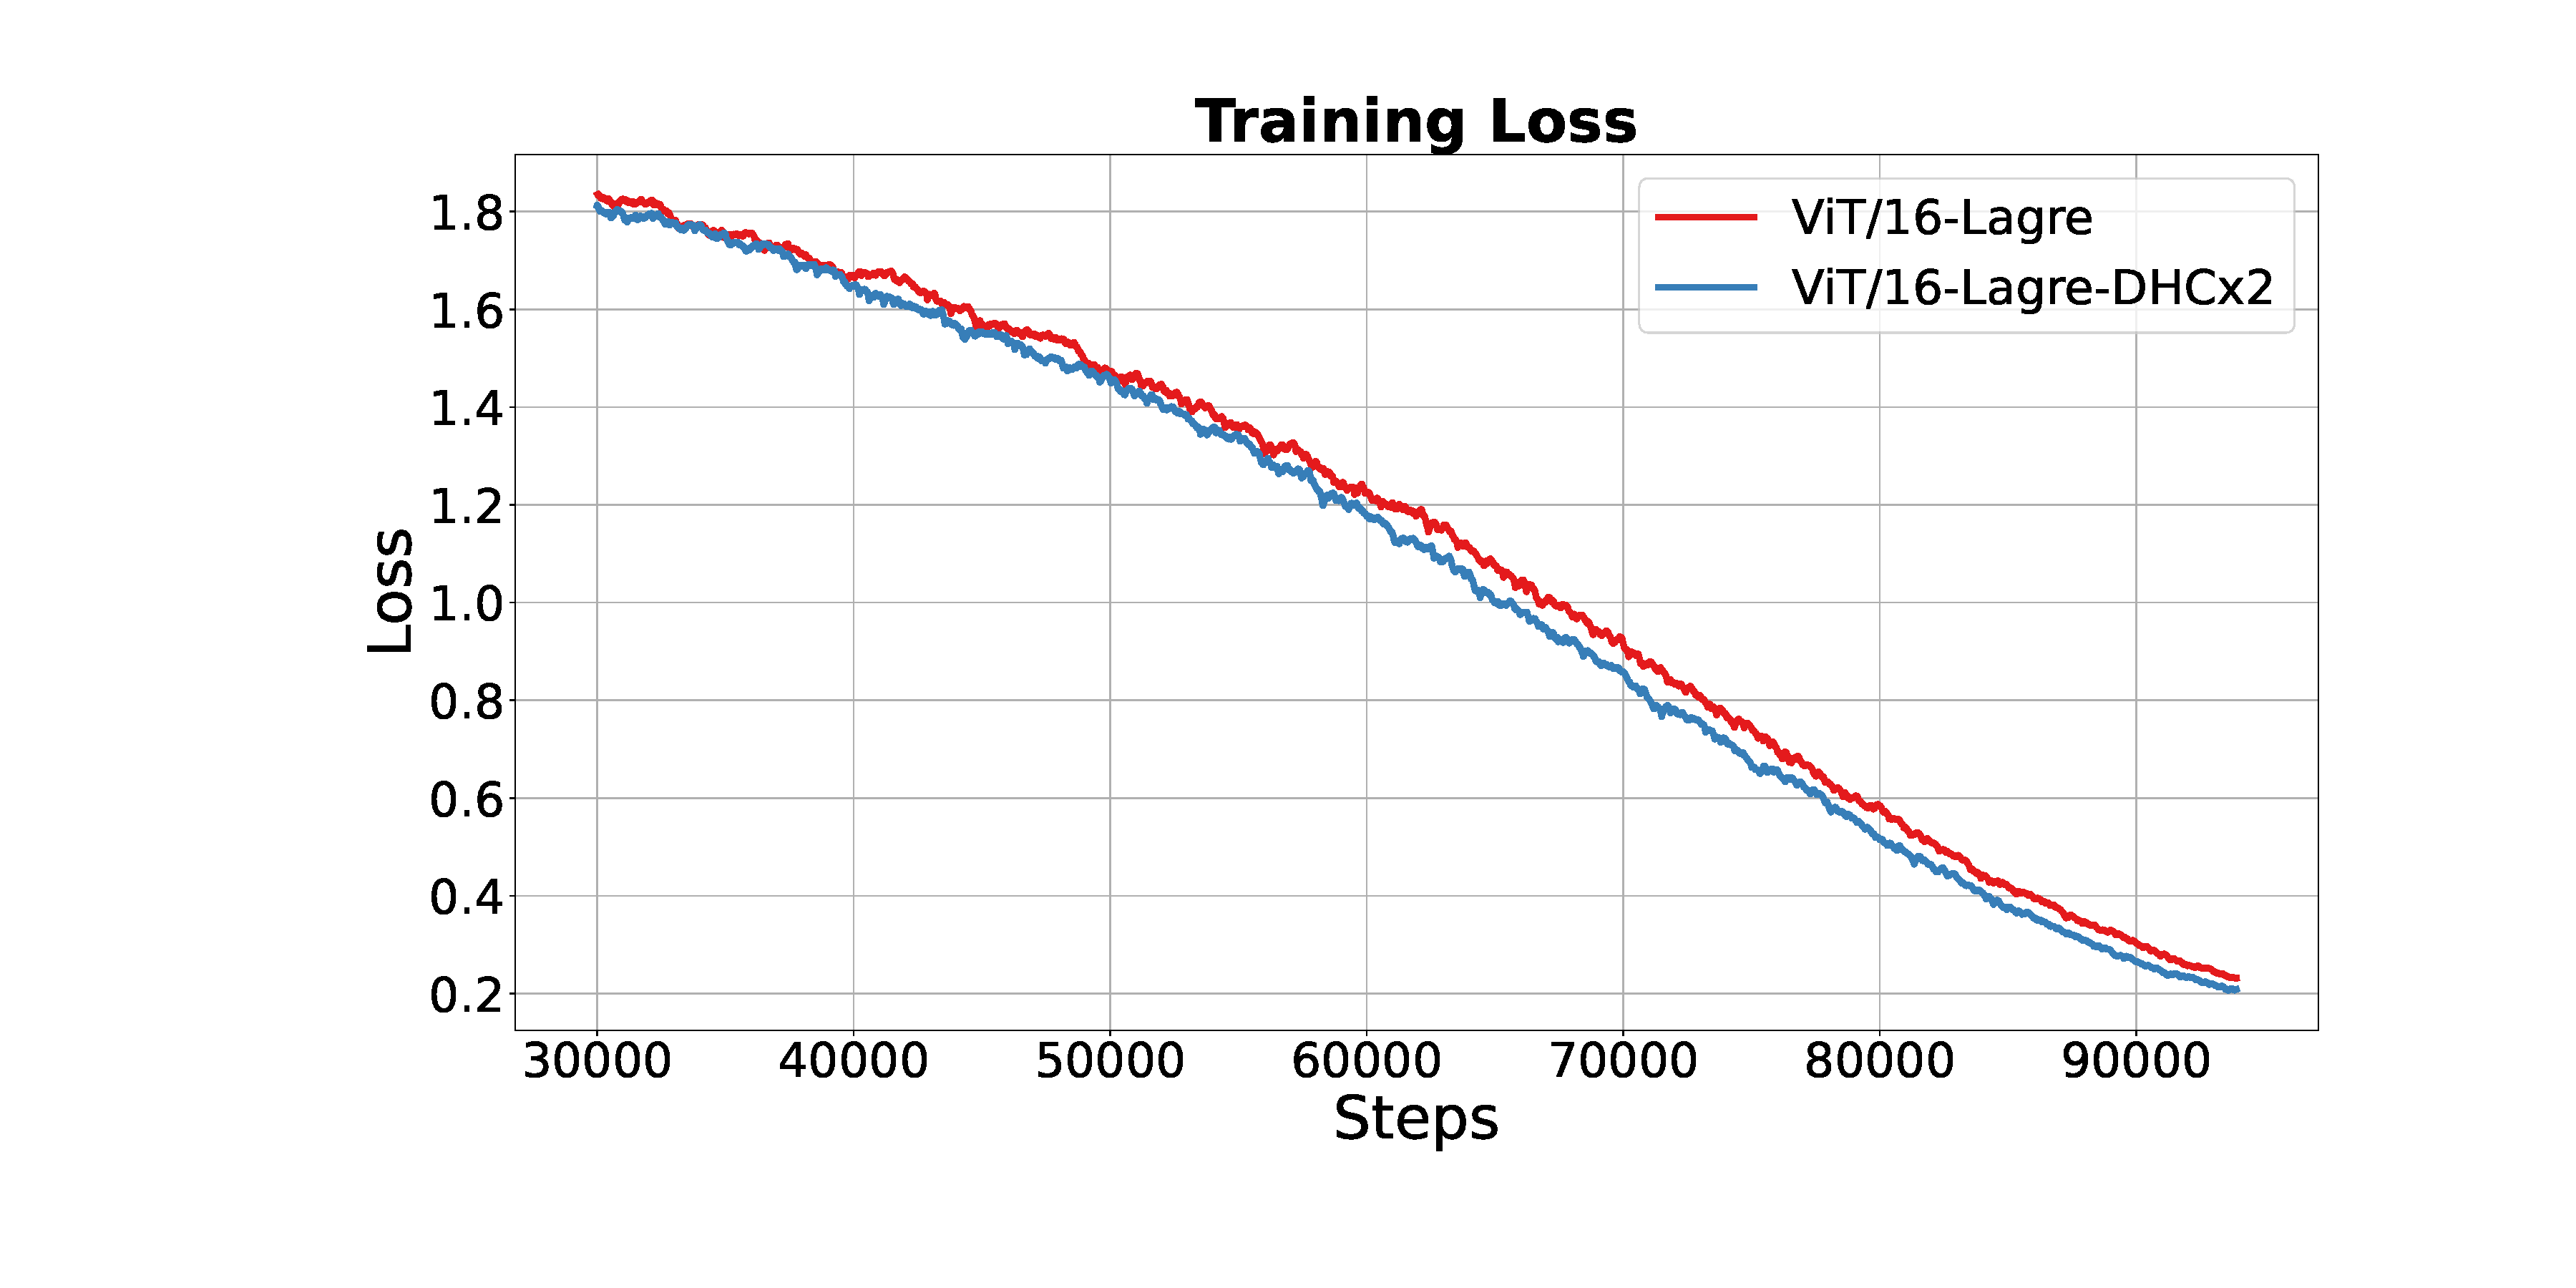
\includegraphics[width=1\textwidth]{fig/train_loss_vitl_exp_0999.pdf}
    \end{center}
  \caption{\newtext{Training loss curves of ViT/16-Large and ViT/16-Large-DHC$\times$2, smoothed using an Exponential Moving Average (EMA) with a decay rate of 0.999. The gain from Hyper-Connections decreases as training progresses, likely due to pass over the same dataset across many epochs, resulting in diminishing returns from the additional capacity provided by Hyper-Connections.}}
    \label{fig:vit_loss}
\end{figure}

\subsection{Visulization of DHC}

\newtext{We randomly select three categories from the ImageNet dataset and sample the corresponding examples from the validation set. These samples are fed into the ViT-Base/16-DHC$\times$2 model to compute the dynamic connection weights of the DHC in the final layer. As shown in Fig.~\ref{fig:vit_last_hc_distribution}, we visualize the distribution of these weights. We observe that the intra-class distribution of beta is highly concentrated, indicating that samples within the same category tend to have similar beta values. In contrast, the distribution of alpha is less concentrated, but the differences between the distributions of different categories are more pronounced, as exemplified by $\alpha_{2,0}$.}

\begin{figure}[h]
    \begin{center}
    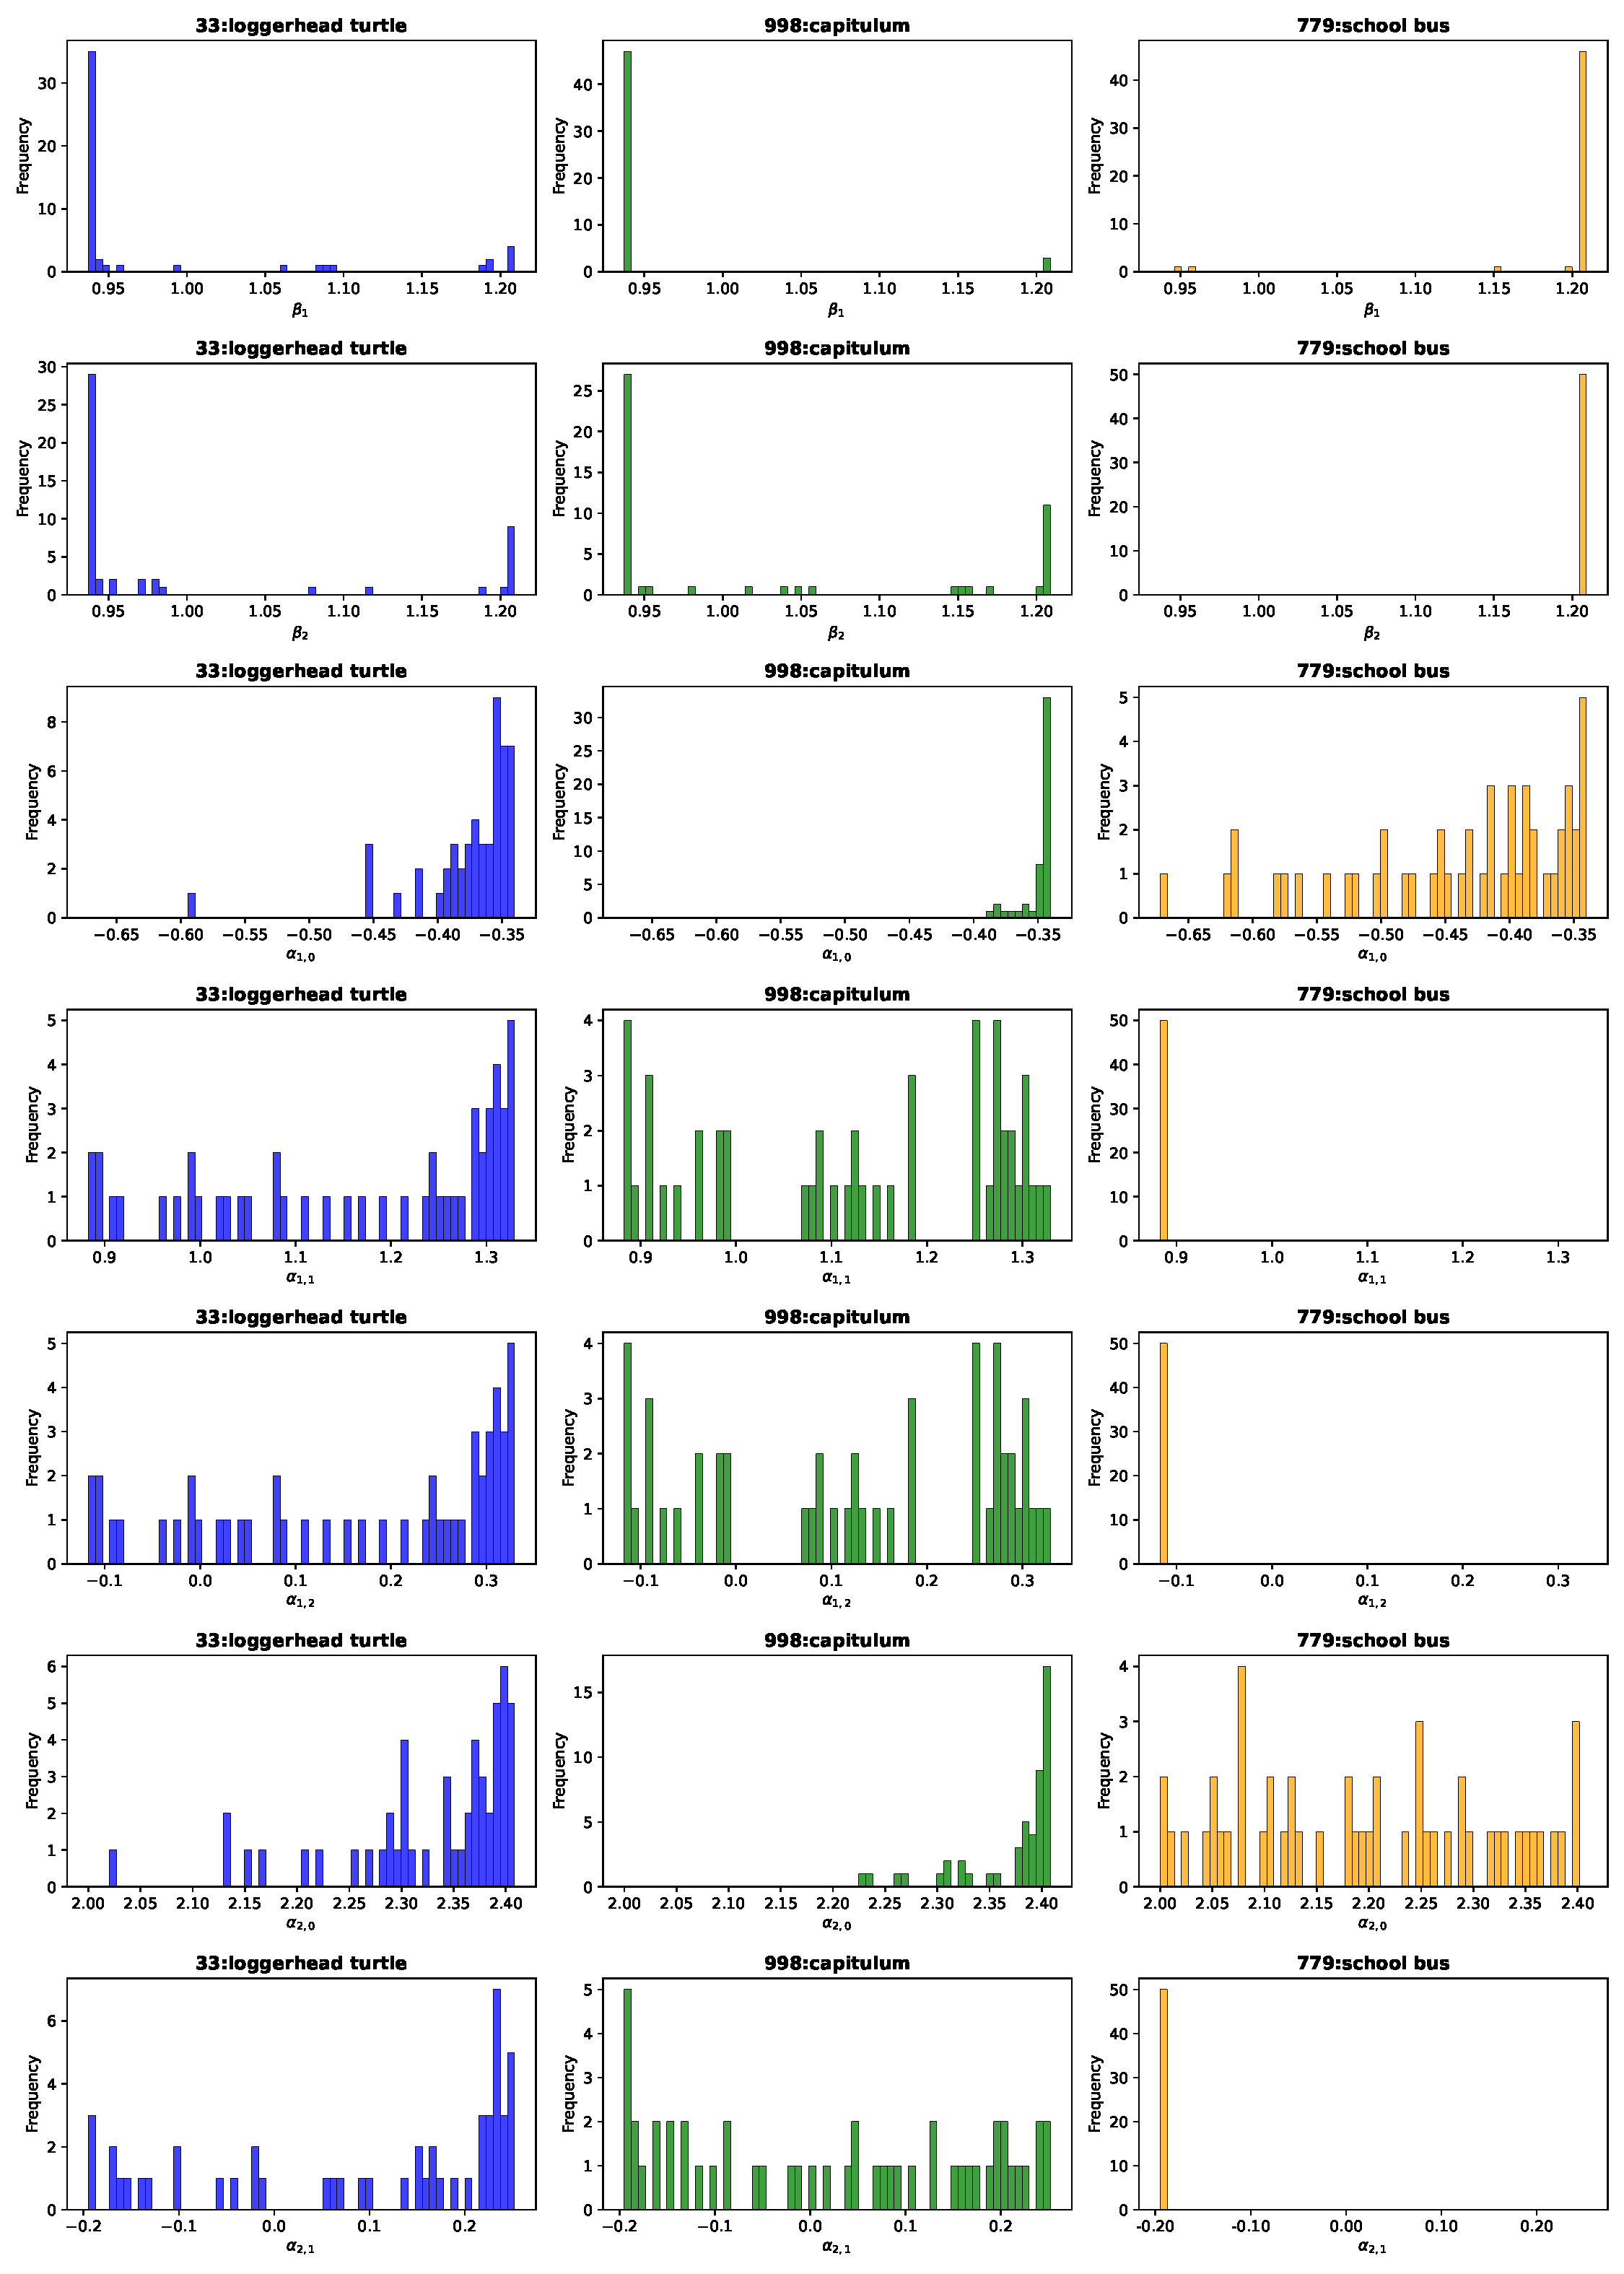
\includegraphics[width=1\textwidth]{fig/distribution_of_hc_final.pdf}
    \end{center}
  \caption{\newtext{Distribution of weights of last DHC in ViT-Base/16-DHC$\times$2 model.}}
    \label{fig:vit_last_hc_distribution}
\end{figure}

\begin{table}[h]
    \centering
    \caption{Training hyperparameters for ViT.}
    \renewcommand{\arraystretch}{1.2} % 增加行间距
    \begin{tabular}{>{\columncolor{gray!20}}l l}
        \toprule
        \cellcolor{lightgray} \textbf{Hyperparameter} & \cellcolor{lightgray} \textbf{Value} \\
        \midrule
        \textbf{Learning Rate (lr)} & 0.003 \\
        \textbf{Batch Size} & 4096 \\
        \textbf{Scheduler} & Cosine Annealing with Linear Warmup (10k steps) \\
        \textbf{Data Augmentation} & Mixup ($\alpha=0.2$) \\
        \textbf{Epochs} & 300 \\
        \textbf{Optimizer} & AdamW ($\beta_1=0.9$, $\beta_2=0.999$, $\epsilon=1e-8$) \\
        \textbf{Gradient Clipping} & 1.0 \\
        \textbf{Weight Decay} & 0.3 \\
        \textbf{Dropout} & 0.1 \\
        \textbf{Precision} & bf16 \\
        \bottomrule
    \end{tabular}
    \label{tab:vit_hyperparameters}
\end{table}

\newpage
\section{More Visualization and Analysis}
\label{app:more_visulization}

\begin{figure*}
    \centering
    \begin{subfigure}{\columnwidth}
        \begin{overpic}[abs,unit=1mm,scale=.25,width=\textwidth]{fig/connection_1Bx4_dyn_token1.pdf}
            \put(17,19){ $\mathbf{C}^{(0)}$} % 在图片上添加公式
            \put(42.5,19){ $\mathbf{C}^{(1)}$} % 在图片上添加公式
            \put(68,19){ $\mathbf{C}^{(2)}$} % 在图片上添加公式
            \put(94,19){ $\mathbf{C}^{(3)}$} % 在图片上添加公式
            \put(120,19){ $\mathbf{C}^{(4)}$} % 在图片上添加公式
        \end{overpic}
        \caption{Connection matrix for DHC model.}
        \label{fig:1bx4_unfold_connection_dhc}
    \end{subfigure}
    
    \begin{subfigure}{\columnwidth}
        \begin{overpic}[abs,unit=1mm,scale=.25,width=\textwidth]{fig/connection_1Bx4_stc.pdf}
            \put(17,19){ $\mathbf{C}^{(0)}$} % 在图片上添加公式
            \put(42.5,19){ $\mathbf{C}^{(1)}$} % 在图片上添加公式
            \put(68,19){ $\mathbf{C}^{(2)}$} % 在图片上添加公式
            \put(94,19){ $\mathbf{C}^{(3)}$} % 在图片上添加公式
            \put(120,19){ $\mathbf{C}^{(4)}$} % 在图片上添加公式
        \end{overpic}
        \caption{Connection matrix for SHC model.}
        \label{fig:1bx4_unfold_connection_shc}
    \end{subfigure}
    \caption{\textbf{Visualization of unfolded connection matrix.} Matrices from left to right are  $\mathbf{C}^{(0)}$(Connections for $\{\mathbf{h}_0^j\}_{j=0}^{L+1}$), $\mathbf{C}^{(i)}$ (Connections for $\{\mathbf{h'}_i^j\}_{j=0}^{L+1}$) for $i\in\{1,2,3,4\}$. The attention layers, which have odd ids, are marked with green tick marks. }
    \label{fig:1bx4_unfold_connection}
\end{figure*}


\paragraph{Unfolding hyper-connections.}
We first introduce how to determine the connection matrix $\mathbf{C}^{(0)}$ for hyper-connections. To simplify writing, the layer output $\mathcal{T}^{k}(\mathbf{h}_0^{k})$ is denoted by $\mathcal{T}^{k}$ for short. The recurrent form of hyper connection in Eq.~\ref{eq:hc_recurrent_form} is expanded as follows:
% \begin{align}
%     {\mathbf{h_0}^{k}}^\intercal=&{\mathbf{A_m}^{k}}^\intercal \mathbf{H}^{k} = {\mathbf{A_r}^{k}}^\intercal ({\mathbf{B}^{k-1}}^\intercal {\mathcal{T}^{k-1}}^\intercal + {\mathbf{A_r}^{k-1}}^\intercal \mathbf{H}^{k-1} ) \notag\\
%     =& \sum_{j=0}^{k-1}{\mathbf{A_r}^{k}}^\intercal({\mathbf{A_{r}}^{k-1}}^\intercal {\mathbf{A_r}^{k-2}}^\intercal ... {\mathbf{A_r}^{j+1}}^\intercal){\mathbf{B}^j}^\intercal {\mathcal{T}^j}^\intercal=\sum_{j=0}^{k-1}{\mathbf{A_r}^{j+1:k}}^\intercal {\mathbf{B}^j}^\intercal {\mathcal{T}^j}^\intercal. \label{eq:expanded_hc}
% \end{align}
\begin{align}
    {\mathbf{h_0}^{k}}=&{\mathbf{H}^{k}}^\intercal \mathbf{A_m}^{k}
    =(\mathcal{T}^{k-1}\mathbf{B}^{k-1} + {\mathbf{H}^{k-1}}^\intercal \mathbf{A_r}^{k-1} )\mathbf{A_m}^{k} \notag\\
    =& \sum_{j=0}^{k-1}\mathcal{T}^j\mathbf{B}^j(\mathbf{A_r}^{j+1}\mathbf{A_r}^{j+2} ... \mathbf{A_{r}}^{k-1})\mathbf{A_m}^{k} \notag \\
    =& \sum_{j=0}^{k-1}\mathcal{T}^j\mathbf{B}^j(\prod_{t=j+1}^{k-1}{\mathbf{A_r}^t})\mathbf{A_m}^{k}. \label{eq:expanded_hc}
\end{align}
Therefore, we obtain connection matrix $c^{(0)}_{kj}=\mathbf{B}^j(\prod_{t=j+1}^{k-1}{\mathbf{A_r}^t})\mathbf{A_m}^{k}$. Similarly, the connection matrix $\mathbf{C}^{(i)}$ for the $i$-th hyper hidden from $k$-th layer can be computed by substituting the last ${\mathbf{A_m}^{k}}$ with $\mathbf{A_r}^{k}$ in Eq.~\ref{eq:expanded_hc}, i.e., 
\begin{gather}
{\mathbf{H'}^{k}}={\mathbf{A_r}^{k}}^\intercal \mathbf{H}^{k}=\sum_{j=0}^{k-1}(\prod_{t=j+1}^{k}{\mathbf{A_r}^t})^\intercal {\mathbf{B}^j}^\intercal {\mathcal{T}^j}^\intercal\\
c^{(i)}_{kj}=\left({(\prod_{t=j+1}^{k}{\mathbf{A_r}^t})}^\intercal {\mathbf{B}^j}^\intercal\right)_{i}.
\end{gather}


\paragraph{Visualization for hyper hidden.}
We visualize connection matrices for hyper hiddens in Fig.~\ref{fig:1bx4_unfold_connection} to reveal how hyper-connection maintains intermediate layer outputs.
First of all, the four hyper hiddens are dissimilar and show completely different connection patterns. Then, we can see outputs from FFN layers are preserved long-termly in hyper hiddens, while attention layers are reserved less. It is also observed that the long-term connections are usually stored in pairs of hyper hiddens, where the connection is positive in one hyper hidden but negative in the other, for example, column 0 and 2 in $\mathbf{C}^{(1)},\mathbf{C}^{(3)}$. With such strategy, these connections can be easily eliminated in the sum-pooling operation before the unembedding layer.

\begin{figure*}
    \centering
    \begin{subfigure}[b]{0.3\textwidth}
        \centering
        \begin{overpic}[abs,unit=1mm,scale=.25,width=\textwidth]{fig/connection_1Bx1_dyn_token1_inp.pdf}
            \put(18.4,16){$\downarrow$ \small wasted}
        \end{overpic}
        \caption{\texttt{OLMo-1B}-DHC$\times 1$}
    \end{subfigure}
    \hfill
    \begin{subfigure}[b]{0.3\textwidth}
        \centering
        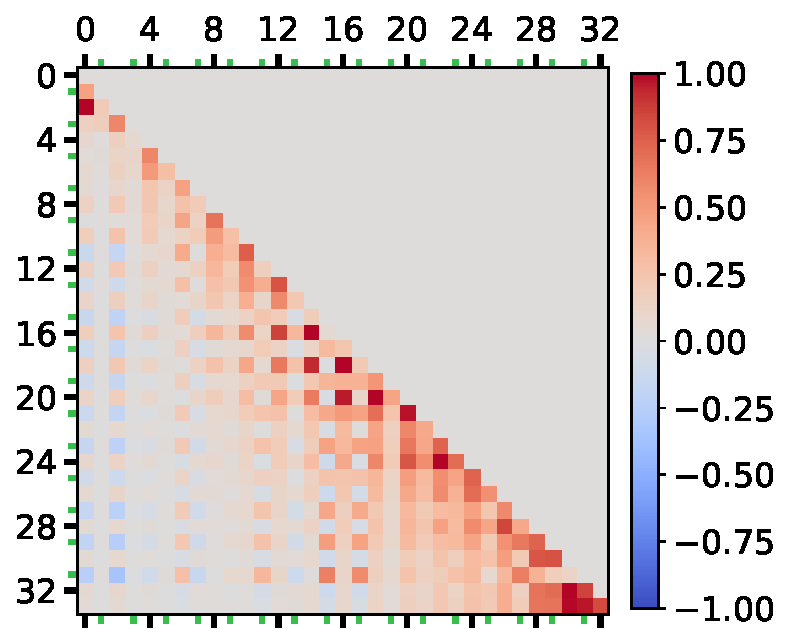
\includegraphics[width=\textwidth]{fig/connection_1Bx2_dyn_token1_inp.pdf}
        \caption{\texttt{OLMo-1B}-DHC$\times 2$}
    \end{subfigure}
    \hfill
    \begin{subfigure}[b]{0.3\textwidth}
        \centering
        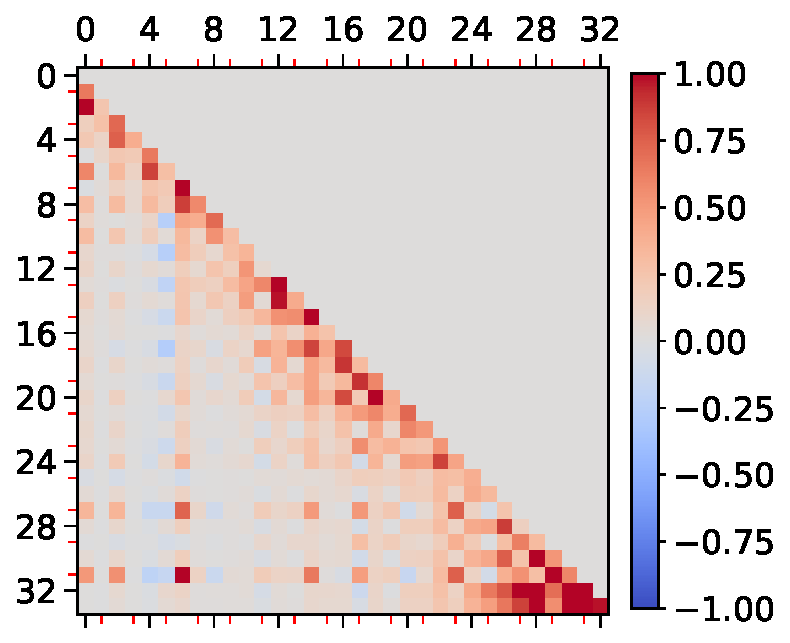
\includegraphics[width=\textwidth]{fig/connection_1Bx4_dyn_token1_inp.pdf}
        \caption{\texttt{OLMo-1B}-DHC$\times 4$}
    \end{subfigure}
    
    \caption{\newtext{Comparison of unfolded connection matrices for \texttt{OLMo-1B}-DHC$\times 1$, \texttt{OLMo-1B}-DHC$\times 2$ and \texttt{OLMo-1B}-DHC$\times 4$ model.}}
    \label{fig:compare_connection_matrix_hcx1}
\end{figure*}


\paragraph{SHC shares similar connection pattern with DHC.} We show the connection matrices for \texttt{OLMo-1B-SHC$\times$4} model in Fig.~\ref{fig:1bx4_unfold_connection_shc}. Comparing to DHC, as shown in Fig.~\ref{fig:1bx4_unfold_connection_dhc}, SHC shares exactly the same connection patterns. Moreover, we observe many more PTB-like blocks in SHC, e.g., layers from 13 to 18. Note that the connection relation for SHC is token independent, and such PTB-like blocks can be physically reorganized to be parallelly computed. 


\paragraph{\newtext{How HC$\times1$ fails.}} \newtext{The \texttt{OLMo-1B}$\times 1$ model is observed to perform worse than baseline in our experiments. Its connection matrix is visualized in Fig.~\ref{fig:compare_connection_matrix_hcx1} to show how it fails. Above all, we observe that layer 17 is wasted, who has no connection to subsequent layers at all. Secondly, compared to HC$\times2$ and HC$\times4$ models, the $\Lambda$ shaped pattern does not appear. Note that HC$\times1$ does not support the pattern of $\Lambda$ in its mathematical formulation, where the connections to previous layers must be weakened or strengthened simultaneously. Thus, the lack of connection from the early layers to the final layers may suffer from gradient vanishing, like post-norm style transformers, which leads to performance degeneration.}

\newpage
\section{Derivation of Non-Trainable Hyper-Connection Matrix for Residual Connections}
\label{app:residual}

\subsection{Pre-Norm Residual Connection}

In the Pre-Norm residual connection, the input to a layer is first normalized before being passed through the layer. The output of the layer is then added to the original input. This can be represented as:

\begin{equation}
    \mathbf{\hat{h}} = \mathcal{T}(\texttt{Norm}(\mathbf{h})) + \mathbf{h}.
\end{equation}

By incorporating the normalization operator into the layer, $\mathcal{T}\coloneqq\mathcal{T}\circ \texttt{Norm}$, we can express the entire process as:
\begin{equation}
    \mathbf{\hat{h}} = \mathcal{T}(\mathbf{h}) + \mathbf{h}.
\end{equation}

To express this using hyper-connections, the matrix for Pre-Norm can be structured as follows:

\begin{equation}
\mathcal{HC}_{PreNorm}=\begin{pmatrix}
0 & 1 \\
1 & 1 \\
\end{pmatrix}
\end{equation}

Given hyper hidden matrix $\mathbf{H}=\mathbf{h}^\intercal$, we prove that the output of $\mathcal{HC}_{\text{PreNorm}}$ $\mathbf{\hat{H}}=\mathbf{\hat{h}}^\intercal$.

\begin{proof}
\begin{equation}
\begin{aligned}
    \mathbf{\hat{H}} &= \mathcal{HC}(\mathcal{T}, \mathbf{H}) \\
                    &=\mathbf{B}^\intercal\mathcal{T}(\mathbf{H}^\intercal\mathbf{A_m})^\intercal + \mathbf{A_r}^\intercal\mathbf{H} \\
                    &=\mathcal{T}(\mathbf{h})^\intercal + \mathbf{h}^\intercal \\
                    &=\mathbf{\hat{h}}^\intercal.
\end{aligned}
\end{equation}
\end{proof}

\subsection{Post-Norm Residual Connection}

In the Post-Norm residual connection, the input to a layer is passed through the layer first, and then the output is normalized after being added to the original input. In matrix form, this can be represented as:

\begin{equation}
\mathbf{h}' = \mathcal{T}(\mathbf{h})
\end{equation}

The summation of the input and the normalized output of the layer is:

\begin{equation}
\mathbf{\hat{h}} = \texttt{Norm}(\mathbf{h} + \mathbf{h}')
\end{equation}


We consider Norm to be LayerNorm~\citep{zhang2019root}. The analysis process for RMSNorm is almost identical. In fact, the affine transformation can be incorporated into the subsequent layer, while the mean subtraction operation can be integrated into the current layer.

\begin{equation}
\mathcal{T} = \mathcal{C} \circ \mathcal{T} \circ \mathcal{A},
\end{equation}
where $\mathcal{A}$ is the affine transformation, and $\mathcal{C}$ is the re-centering operator. Thus, the mean of the output of $\mathcal{T}$ is $0$.

To express this using hyper-connections with an expansion rate $n=1$, we need a hyper-connection matrix $\mathcal{HC}$ that encapsulates this operation:

\begin{equation}
\mathcal{HC}_{PostNorm}=\begin{pmatrix}
0 & \frac{1}{\sqrt{\sigma_{\mathbf{h}}^2 + \sigma_{\mathbf{h}'}^2 + 2\sigma_{\mathbf{h}\mathbf{h}'}}} \\
1 & \frac{1}{\sqrt{\sigma_{\mathbf{h}}^2 + \sigma_{\mathbf{h}'}^2 + 2\sigma_{\mathbf{h}\mathbf{h}'}}} \\
\end{pmatrix}=\begin{pmatrix}
0 & \mathbf{B} \\
\mathbf{A}_m & \mathbf{A}_r \\
\end{pmatrix}.
\end{equation}

Similar to the previous proof, we prove that the output of $\mathcal{HC}_{\text{PostNorm}}$ is equivalent to the transpose of the output of the Post-Norm residual connection: 
\begin{equation}
    \mathbf{\hat{H}}=\mathbf{\hat{h}}^\intercal.
\end{equation}

\begin{proof}
Note that

\begin{equation}
\sigma_{\mathbf{h} + \mathbf{h}'} = \sqrt{\sigma_{\mathbf{h}}^2 + \sigma_{\mathbf{h}'}^2 + 2\sigma_{\mathbf{h}\mathbf{h}'}}.
\end{equation}

Given this fact, we can derive the Post-Norm:

\begin{equation}
\begin{aligned}
     \mathbf{\hat{h}} &= \text{Norm}(\mathbf{h}' + \mathbf{h}) \\
    &= \frac{\mathbf{h}' + \mathbf{h} - \mu_{\mathbf{h}' + \mathbf{h}}}{\sigma_{\mathbf{h} + \mathbf{h}'}} \\
    &= \frac{1}{\sigma_{\mathbf{h}' + \mathbf{h}}} (\mathbf{h}' + \mathbf{h}) \\
    &= \frac{1}{\sqrt{\sigma_{\mathbf{h}}^2 + \sigma_{\mathbf{h}'}^2 + 2\sigma_{\mathbf{h}\mathbf{h}'}}} (\mathbf{h}' + \mathbf{h})
\end{aligned}
\end{equation}

For hyper-connections side, we have:
\begin{equation}
\begin{aligned}
    \mathbf{\hat{H}} &= \mathbf{B}^\intercal \mathbf{h}'^\intercal + \mathbf{H}' \\
    &= \mathbf{B}^\intercal \mathbf{h}'^\intercal + \mathbf{A}_r \mathbf{H} \\
    &= \mathbf{B}^\intercal \mathbf{h}'^\intercal + \mathbf{A}_r \mathbf{h}^\intercal \\
    &= \frac{1}{\sqrt{\sigma_{\mathbf{h}}^2 + \sigma_{\mathbf{h}'}^2 + 2\sigma_{\mathbf{h}\mathbf{h}'}}} \mathbf{h}'^\intercal + 
    \frac{1}{\sqrt{\sigma_{\mathbf{h}}^2 + \sigma_{\mathbf{h}'}^2 + 2\sigma_{\mathbf{h}\mathbf{h}'}}} \mathbf{h}^\intercal
    &= \mathbf{\hat{h}}^\intercal.
\end{aligned}
\end{equation}

\end{proof}


\newpage
\section{Sequential-Parallel Duality}
\label{app:spd}
\subsection{Hyper-Connection Matrix of Sequential Arrangement}
In this section, we demonstrate that the following hyper-connection matrix will produce $n$ identical networks arranged sequentially with residual connections between them:

\begin{equation}
\label{eq:nxn_sequential}
\mathcal{HC}=\begin{pmatrix}
\mathbf{0}_{1 \times 1} & \mathbf{1}_{1 \times n}\\
\mathbf{e}_1 & \mathbf{e}_{n\times n}
\end{pmatrix},
\end{equation}
where $\mathbf{e}_{n\times n}$ denotes an $n \times n$ identity matrix, $\mathbf{e}_i \in \mathbb{R}^{n \times 1}$ represents the $i$-th column of $\mathbf{e}_{n\times n}$, and $\mathbf{1}_{1 \times n}$ signifies a $1 \times n$ matrix of ones.

We will use mathematical induction to prove that $\mathbf{h}_i^k = \mathbf{h}_j^k$ and $\mathbf{h}_i^{k+1} = \mathcal{T}^k(\mathbf{h}_i^k) + \mathbf{h}_i^k$, $\forall i,j \in \{0, 1, \ldots, n\}$, $\forall k \in \{0, 1, \ldots, L\}$, where $L$ is the number of layers.

\begin{proof}
\subsection*{Base Case}
For $k = 0$, we have the initial condition $\mathbf{h}_i^0 = \mathbf{h}_j^0$, $\forall i, j \in \{0, 1, \ldots, n\}$, as we define $\mathbf{H}^0 = \begin{pmatrix} \mathbf{h}^0 & \mathbf{h}^0 & \dots & \mathbf{h}^0 \end{pmatrix}^\intercal \in \mathbb{R}^{n \times d}$.

\subsection*{Induction Hypothesis}
Assume that for some $k \in \{1, \ldots, L-1\}$, we have $\mathbf{h}_i^k = \mathbf{h}_j^k$ and $\mathbf{h}_i^k = \mathcal{T}^k(\mathbf{h}_i^{k-1}) + \mathbf{h}_i^{k-1}$, $\forall i, j \in \{0, 1, \ldots, n\}$.

\subsection*{Induction Step}
We have

\begin{align}
\mathbf{H}^{k+1} &= \mathcal{HC}(\mathcal{T}^k, \mathbf{H}^k) \\
&= \mathbf{B}^\intercal (\mathbf{h}'^{k}_0)^\intercal + \mathbf{H'}^k \\
&= \mathbf{B}^\intercal \mathbf{A_m}^\intercal \mathbf{H}^k + \mathbf{A_r}^\intercal \mathbf{H}^k \\
&= \mathbf{1}_{n \times 1} \mathcal{T}^k (\mathbf{e}_1^\intercal \mathbf{H}^k) + \mathbf{e}_{n \times n} \mathbf{H}^k \\
&= \begin{pmatrix}
\mathcal{T}^k(\mathbf{h}_1^k) & \mathcal{T}^k(\mathbf{h}_1^k) & \ldots & \mathcal{T}^k(\mathbf{h}_1^k)
\end{pmatrix}^\intercal + \begin{pmatrix} 
\mathbf{h}_1^k & \mathbf{h}_2^k & \dots & \mathbf{h}_n^k 
\end{pmatrix}^\intercal \\
&= \begin{pmatrix}
\mathcal{T}^k(\mathbf{h}_1^k) + \mathbf{h}_1^k & 
\mathcal{T}^k(\mathbf{h}_1^k) + \mathbf{h}_2^k &
\ldots &
\mathcal{T}^k(\mathbf{h}_1^k) + \mathbf{h}_n^k
\end{pmatrix}^\intercal \\
&= \begin{pmatrix} 
\mathbf{h}_1^{k+1} & \mathbf{h}_2^{k+1} & \dots & \mathbf{h}_n^{k+1} 
\end{pmatrix}^\intercal
\end{align}

Since $\mathbf{h}_i^k = \mathbf{h}_j^k$, $\forall i, j \in \{0, 1, \ldots, n\}$, it follows that $\mathcal{T}^k(\mathbf{h}_1^k) + \mathbf{h}_i^k = \mathcal{T}^k(\mathbf{h}_1^k) + \mathbf{h}_j^k$. Thus, we have

\begin{equation}
\mathbf{h}_i^{k+1} = \mathbf{h}_j^{k+1}
\end{equation}

Since $\mathbf{h}_i^k = \mathbf{h}_j^k$, $\forall i, j \in \{0, 1, \ldots, n\}$, it follows that $\mathbf{h}_1^k = \mathbf{h}_i^k$, $\forall i \in \{0, 1, \ldots, n\}$. Thus, we have

\begin{align}
\mathbf{h}_i^{k+1} &= \mathcal{T}^k(\mathbf{h}_1^k) + \mathbf{h}_i^k \\
&= \mathcal{T}^k(\mathbf{h}_i^k) + \mathbf{h}_i^k
\end{align}
\end{proof}

\subsection{Hyper-Connection Matrix of Parallel Arrangement}
In this section, we demonstrate that the following hyper-connection matrix will produce a network where every $n$ adjacent layers are arranged in parallel, with each layer incorporating residual connections.
We define a parallel-arranged network such that $n$ adjacent layers form a group, with layers within a group being parallel and groups arranged sequentially. The output of $k$-th group is given by:

\begin{equation}
\mathbf{h}^{k+1}=\sum_{i=1}^{n}(\mathcal{T}^{k\times n+i}(\mathbf{h}^{k}) + \mathbf{h}^k).
\end{equation}

It can be proved that this arrangement can be described by the following hyper-connection matrices.

\textbf{First, for $k$ where $k-1 \equiv 0 \pmod{n}$:}

\begin{equation}
\mathcal{HC}^{\{ k \mid k-1 \equiv 0 \pmod{n} \}}=
  \begin{pmatrix}
  \mathbf{0}_{1\times 1} & \mathbf{e}_1^\intercal \\
  \mathbf{1}_{n\times 1} & \mathbf{1}_{n\times n},
  \end{pmatrix}
\end{equation}

where the $\mathcal{HC}$ matrix can be decomposed into two operations: 1) sum up all the outputs of the previous group and use it as the input of the current layer and as the residual of the subsequent layers; 2) sum up the output and input saving to the first hidden vector slot.

\textbf{Next, for $k$ where $k-1 \equiv i \pmod{n}$ and $i \neq 0$:}

\begin{equation}
\mathcal{HC}^{\{ k \mid k-1 \equiv i \pmod{n}, i \neq 0 \}}=
  \begin{pmatrix}
  \mathbf{0}_{1\times 1} & \mathbf{e}_i^\intercal \\
  \mathbf{e}_i & \mathbf{e}_{n\times n}, 
  \end{pmatrix}.
\end{equation}

where the \(\mathcal{HC}\) matrix selects the \( i \)-th hidden vector as the input of the current layer, and sums up the output and input, saving to the \( i \)-th hidden vector slot.

This means: 
\begin{align}
\mathbf{h}^{k+1}=&\mathcal{HC}^{(k+1)\times n}(\mathcal{T}^{(k+1)\times n}, \\
&\mathcal{HC}^{(k+1)\times n - 1}(\mathcal{T}^{(k+1)\times n - 1}, \\
&\cdots  \\
&\mathcal{HC}^{k\times n+1}(\mathcal{T}^{k\times n+1},\mathbf{h}^{k})))
\end{align}

This can also be proved by mathematical induction; however, the conclusion is quite obvious through drawing, and the proof process is very tedious. Therefore, we don't repeat the similar proof here.


\newpage
\section{Pseudocode of Hyper-connections}

\begin{algorithm}[h]
\caption{Network with Hyper-Connections}\label{alg:hyper_connections}
\begin{algorithmic}[1]
\Require Initial hidden vector $\mathbf{h}^0 \in \mathbb{R}^d$
\Require Expansion rate $n$
\Ensure Final output $\mathbf{y}$

\State \textbf{Initialize:}
\State $\mathbf{H}^0 \gets \begin{pmatrix} \mathbf{h}^0 & \mathbf{h}^0 & \dots & \mathbf{h}^0 \end{pmatrix}^\intercal \in \mathbb{R}^{n\times d}$

\For{$k = 1$ to $L$} \Comment{For each layer}
    \State $\mathbf{H} \gets \mathbf{H}^{k-1}$
    
    \State $\begin{pmatrix} \mathbf{h}_0 & \mathbf{H'} \end{pmatrix} \gets \mathcal{WC}^{k\intercal} \mathbf{H}$ \Comment{Width Connections}
    
    \State $\mathbf{h}'_0 \gets \mathcal{T}^k(\mathbf{h}_0)$ \Comment{Layer Computation}
    
    \State $\mathbf{\hat{H}} \gets \mathbf{B}^{k\intercal} \mathbf{h}'_0 + \mathbf{H'}$ \Comment{Depth Connections}
    
    \State $\mathbf{H}^k \gets \mathbf{\hat{H}}$
\EndFor

\State \textbf{Final Output:}
\State $\mathbf{h}^L \gets \text{sum rows of } \mathbf{H}^L$
\State $\mathbf{h}^L \gets \text{Normalization Layer}(\mathbf{h}^L)$
\State $\mathbf{y} \gets \text{Output Layer}(\mathbf{h}^L)$

\State \Return $\mathbf{y}$
\end{algorithmic}
\end{algorithm}

\label{app:pytorch}

\newpage
\section{PyTorch Implementation of Hyper-connections}
\begin{algorithm}[h]
\caption{Pseudocode of hyper-connections in a PyTorch-like style.}
\label{alg:torch_hc}
\algcomment{\fontsize{7.2pt}{0em}\selectfont 
%\vspace{-1.em}
}
\definecolor{codeblue}{rgb}{0.25,0.5,0.5}
\lstset{
  backgroundcolor=\color{white},
  basicstyle=\fontsize{7.2pt}{7.2pt}\ttfamily\selectfont,
  columns=fullflexible,
  breaklines=true,
  captionpos=b,
  commentstyle=\fontsize{7.2pt}{7.2pt}\color{codeblue},
  keywordstyle=\fontsize{7.2pt}{7.2pt},
%  frame=tb,
}
\begin{lstlisting}[language=python]
# h: hyper hidden matrix (BxLxNxD)

class HyperConnection(nn.Module):
    def __init__(self, dim, rate, layer_id, dynamic, device=None):
        super(HyperConnection, self).__init__()

        self.rate = rate
        self.layer_id = layer_id
        self.dynamic = dynamic

        self.static_beta = nn.Parameter(torch.ones((rate,), device=device))

        init_alpha0 = torch.zeros((rate, 1), device=device)
        init_alpha0[layer_id % rate, 0] = 1.
        self.static_alpha = nn.Parameter(torch.cat([init_alpha0, torch.eye((rate), device=device)], dim=1))
       
        if self.dynamic:
            self.dynamic_alpha_fn = nn.Parameter(torch.zeros((dim, rate+1), device=device))
            self.dynamic_alpha_scale = nn.Parameter(torch.ones(1, device=device) * 0.01)
            self.dynamic_beta_fn = nn.Parameter(torch.zeros((dim, ), device=device))
            self.dynamic_beta_scale = nn.Parameter(torch.ones(1, device=device) * 0.01)
            self.layer_norm = LayerNorm(dim)
    
    def width_connection(self, h):
        # get alpha and beta
        if self.dynamic:
            norm_h = self.layer_norm(h)
        
        if self.dynamic:
            wc_weight = norm_h @ self.dynamic_alpha_fn
            wc_weight = F.tanh(wc_weight)
            dynamic_alpha = wc_weight  * self.dynamic_alpha_scale
            alpha = dynamic_alpha + self.static_alpha[None, None, ...]
        else:
            alpha = self.static_alpha[None, None, ...]

        if self.dynamic:
            dc_weight = norm_h @ self.dynamic_beta_fn
            dc_weight = F.tanh(dc_weight)
            dynamic_beta = dc_weight * self.dynamic_beta_scale
            beta = dynamic_beta + self.static_beta[None, None, ...]
        else:
            beta = self.static_beta[None, None, ...]

        # width connection
        mix_h = alpha.transpose(-1, -2)  @  h

        return mix_h, beta
    
    def depth_connection(self, mix_h, h_o, beta):
        h = torch.einsum("blh,bln->blnh", h_o, beta) + mix_h[..., 1:, :]

        return h
\end{lstlisting}
\end{algorithm}

\begin{algorithm}[h]
\caption{Pseudocode of transformer with hyper-connections in a PyTorch-like style.}
\label{alg:torch_trans_with_hc}
\algcomment{\fontsize{7.2pt}{0em}\selectfont 
%\vspace{-1.em}
}
\definecolor{codeblue}{rgb}{0.25,0.5,0.5}
\lstset{
  backgroundcolor=\color{white},
  basicstyle=\fontsize{7.2pt}{7.2pt}\ttfamily\selectfont,
  columns=fullflexible,
  breaklines=true,
  captionpos=b,
  commentstyle=\fontsize{7.2pt}{7.2pt}\color{codeblue},
  keywordstyle=\fontsize{7.2pt}{7.2pt},
%  frame=tb,
}
\begin{lstlisting}[language=python]
# h: hyper hidden matrix (BxLxNxD)
# atten_hyper_connection, ffn_hyper_connection:  hyper-connection modules
# attn_norm, ffn_norm: normalization modules

# Attention Block
mix_h, beta = atten_hyper_connection.width_connection(h)
h = attn_norm(mix_h[...,0,:])
h = self_attention(h)
h = atten_hyper_connection.depth_connection(mix_h, dropout(h), beta)

# FFN Block
mix_h, beta = ffn_hyper_connection.width_connection(h)
h = ffn_norm(mix_h[...,0,:])
h = ffn(h)
h = ffn_hyper_connection.depth_connection(mix_h, dropout(h), beta)

\end{lstlisting}
\end{algorithm}

\newpage

\section{Validation Sets and Downstream Tasks}
\begin{table}[h]
\caption{OLMo's default configuration was evaluated using multiple metrics. Perplexity (PPL) and loss were used for the V2 and V3 Validation Sets, while zero-shot testing was applied to the Downstream Benchmarks. However, the grey benchmarks were excluded from our analysis due to the instability of their performance indicators.}
\centering
\begin{tabular}{|l|}
\hline
\multicolumn{1}{|c|}{\textbf{V2 Validation Sets}} \\
\hline
\texttt{v2-small-4chan-validation} \\
\texttt{v2-small-c4\_100\_domains-validation} \\
\texttt{v2-small-c4\_en-validation} \\
\texttt{v2-small-gab-validation} \\
\texttt{v2-small-ice-validation} \\
\texttt{v2-small-m2d2\_s2orc-validation} \\
\texttt{v2-small-m2d2\_wiki-validation} \\
\texttt{v2-small-manosphere-validation} \\
\texttt{v2-small-mc4\_en-validation} \\
\texttt{v2-small-pile-validation} \\
\texttt{v2-small-ptb-validation} \\
\texttt{v2-small-twitterAEE-validation} \\
\texttt{v2-small-wikitext\_103-validation} \\
\hline
\multicolumn{1}{|c|}{\textbf{V3 Validation Sets}} \\
\hline
\texttt{v3-small-c4\_en-validation} \\
\texttt{v3-small-dolma\_books-validation} \\
\texttt{v3-small-dolma\_common-crawl-validation} \\
\texttt{v3-small-dolma\_pes2o-validation} \\
\texttt{v3-small-dolma\_reddit-validation} \\
\texttt{v3-small-dolma\_stack-validation} \\
\texttt{v3-small-dolma\_wiki-validation} \\
\texttt{v3-small-ice-validation} \\
\texttt{v3-small-m2d2\_s2orc-validation} \\
\texttt{v3-small-pile-validation} \\
\texttt{v3-small-wikitext\_103-validation} \\
\hline
\multicolumn{1}{|c|}{\textbf{Downstream Benchmarks}} \\
\hline
\texttt{piqa}~\citep{bisk2020piqa} \\
\texttt{hellaswag}~\citep{zellers2019hellaswag} \\
\texttt{winogrande}~\citep{sakaguchi2021winogrande} \\
\texttt{openbook\_qa}~\citep{OpenBookQA2018} \\
\texttt{sciq}~\citep{SciQ} \\
\texttt{arc\_easy}~\citep{allenai:arc} \\
\texttt{copa}~\citep{roemmele2011choice} \\
\color{gray}{\texttt{commitment\_bank}~\citep{de2019commitmentbank}} \\
\color{gray}{\texttt{mrpc}~\citep{dolan2005automatically}} \\
\color{gray}{\texttt{rte}~\citep{dagan2005pascal}} \\
\color{gray}{\texttt{sst2}~\citep{socher2013recursive}} \\
\hline
\end{tabular}
\label{tab:combined-sets-benchmarks}
\end{table}

\begin{table}[h]
\centering
\caption{Downstream Benchmarks for OLMoE.}
\begin{tabular}{|l|}
\hline
\multicolumn{1}{|c|}{\textbf{Downstream Benchmarks for OLMoE}} \\
\hline
\texttt{piqa}~\citep{bisk2020piqa} \\
\texttt{hellaswag}~\citep{zellers2019hellaswag} \\
\texttt{winogrande}~\citep{sakaguchi2021winogrande} \\
\texttt{openbook\_qa}~\citep{OpenBookQA2018} \\
\texttt{sciq}~\citep{SciQ} \\
\texttt{arc\_easy}~\citep{allenai:arc} \\
\texttt{arc\_challenage}~\citep{allenai:arc} \\
\texttt{copa}~\citep{roemmele2011choice} \\
\texttt{boolq}~\citep{clark2019boolq} \\
\texttt{commonsense\_qa}~\citep{talmor2018commonsenseqa} \\
\texttt{social\_iqa}~\citep{sap2019socialiqa} \\
\texttt{mmlu}~\citep{hendryckstest2021} \\
\hline
\end{tabular}
\label{tab:olmoe-benchmarks}
\end{table}

\newpage
\section{1B Model Experiments}

\begin{figure}[h]
    \begin{center}
    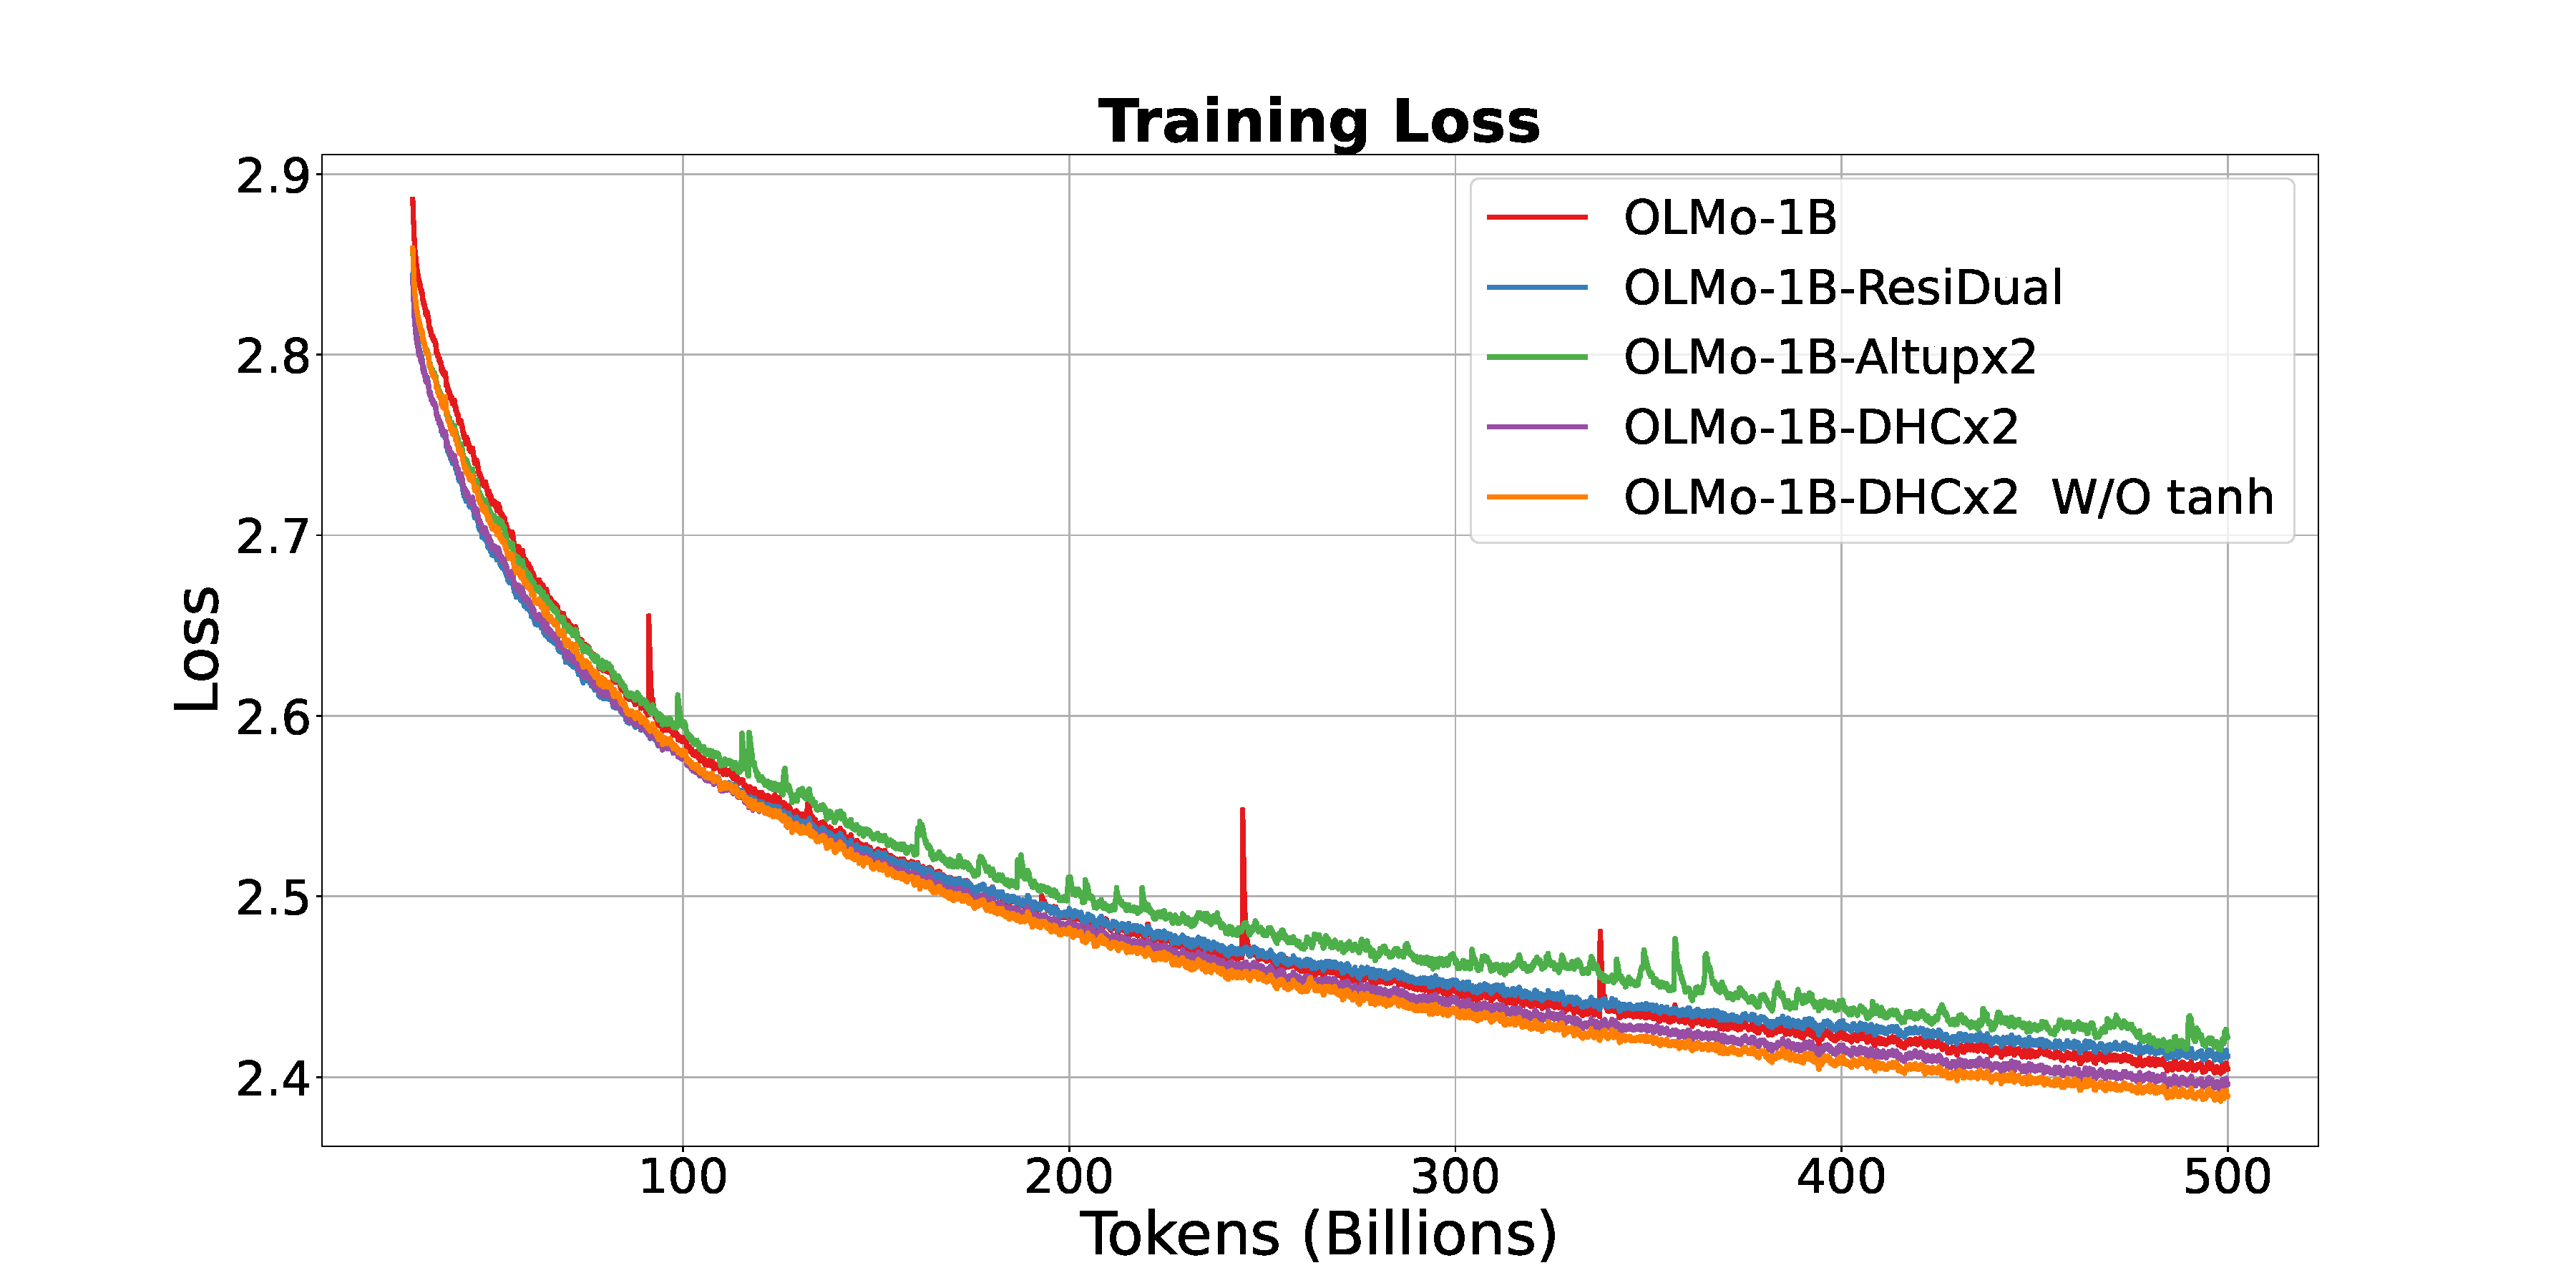
\includegraphics[width=1\textwidth]{fig/train_loss_olmo_related_exp_099.pdf}
    \end{center}
  \caption{\newtext{Training loss curves of related works, smoothed using Exponential Moving Average (EMA) with a decay rate of 0.99.}}
    \label{fig:related_method_loss}
\end{figure}

\begin{figure}[h]
    \begin{center}
    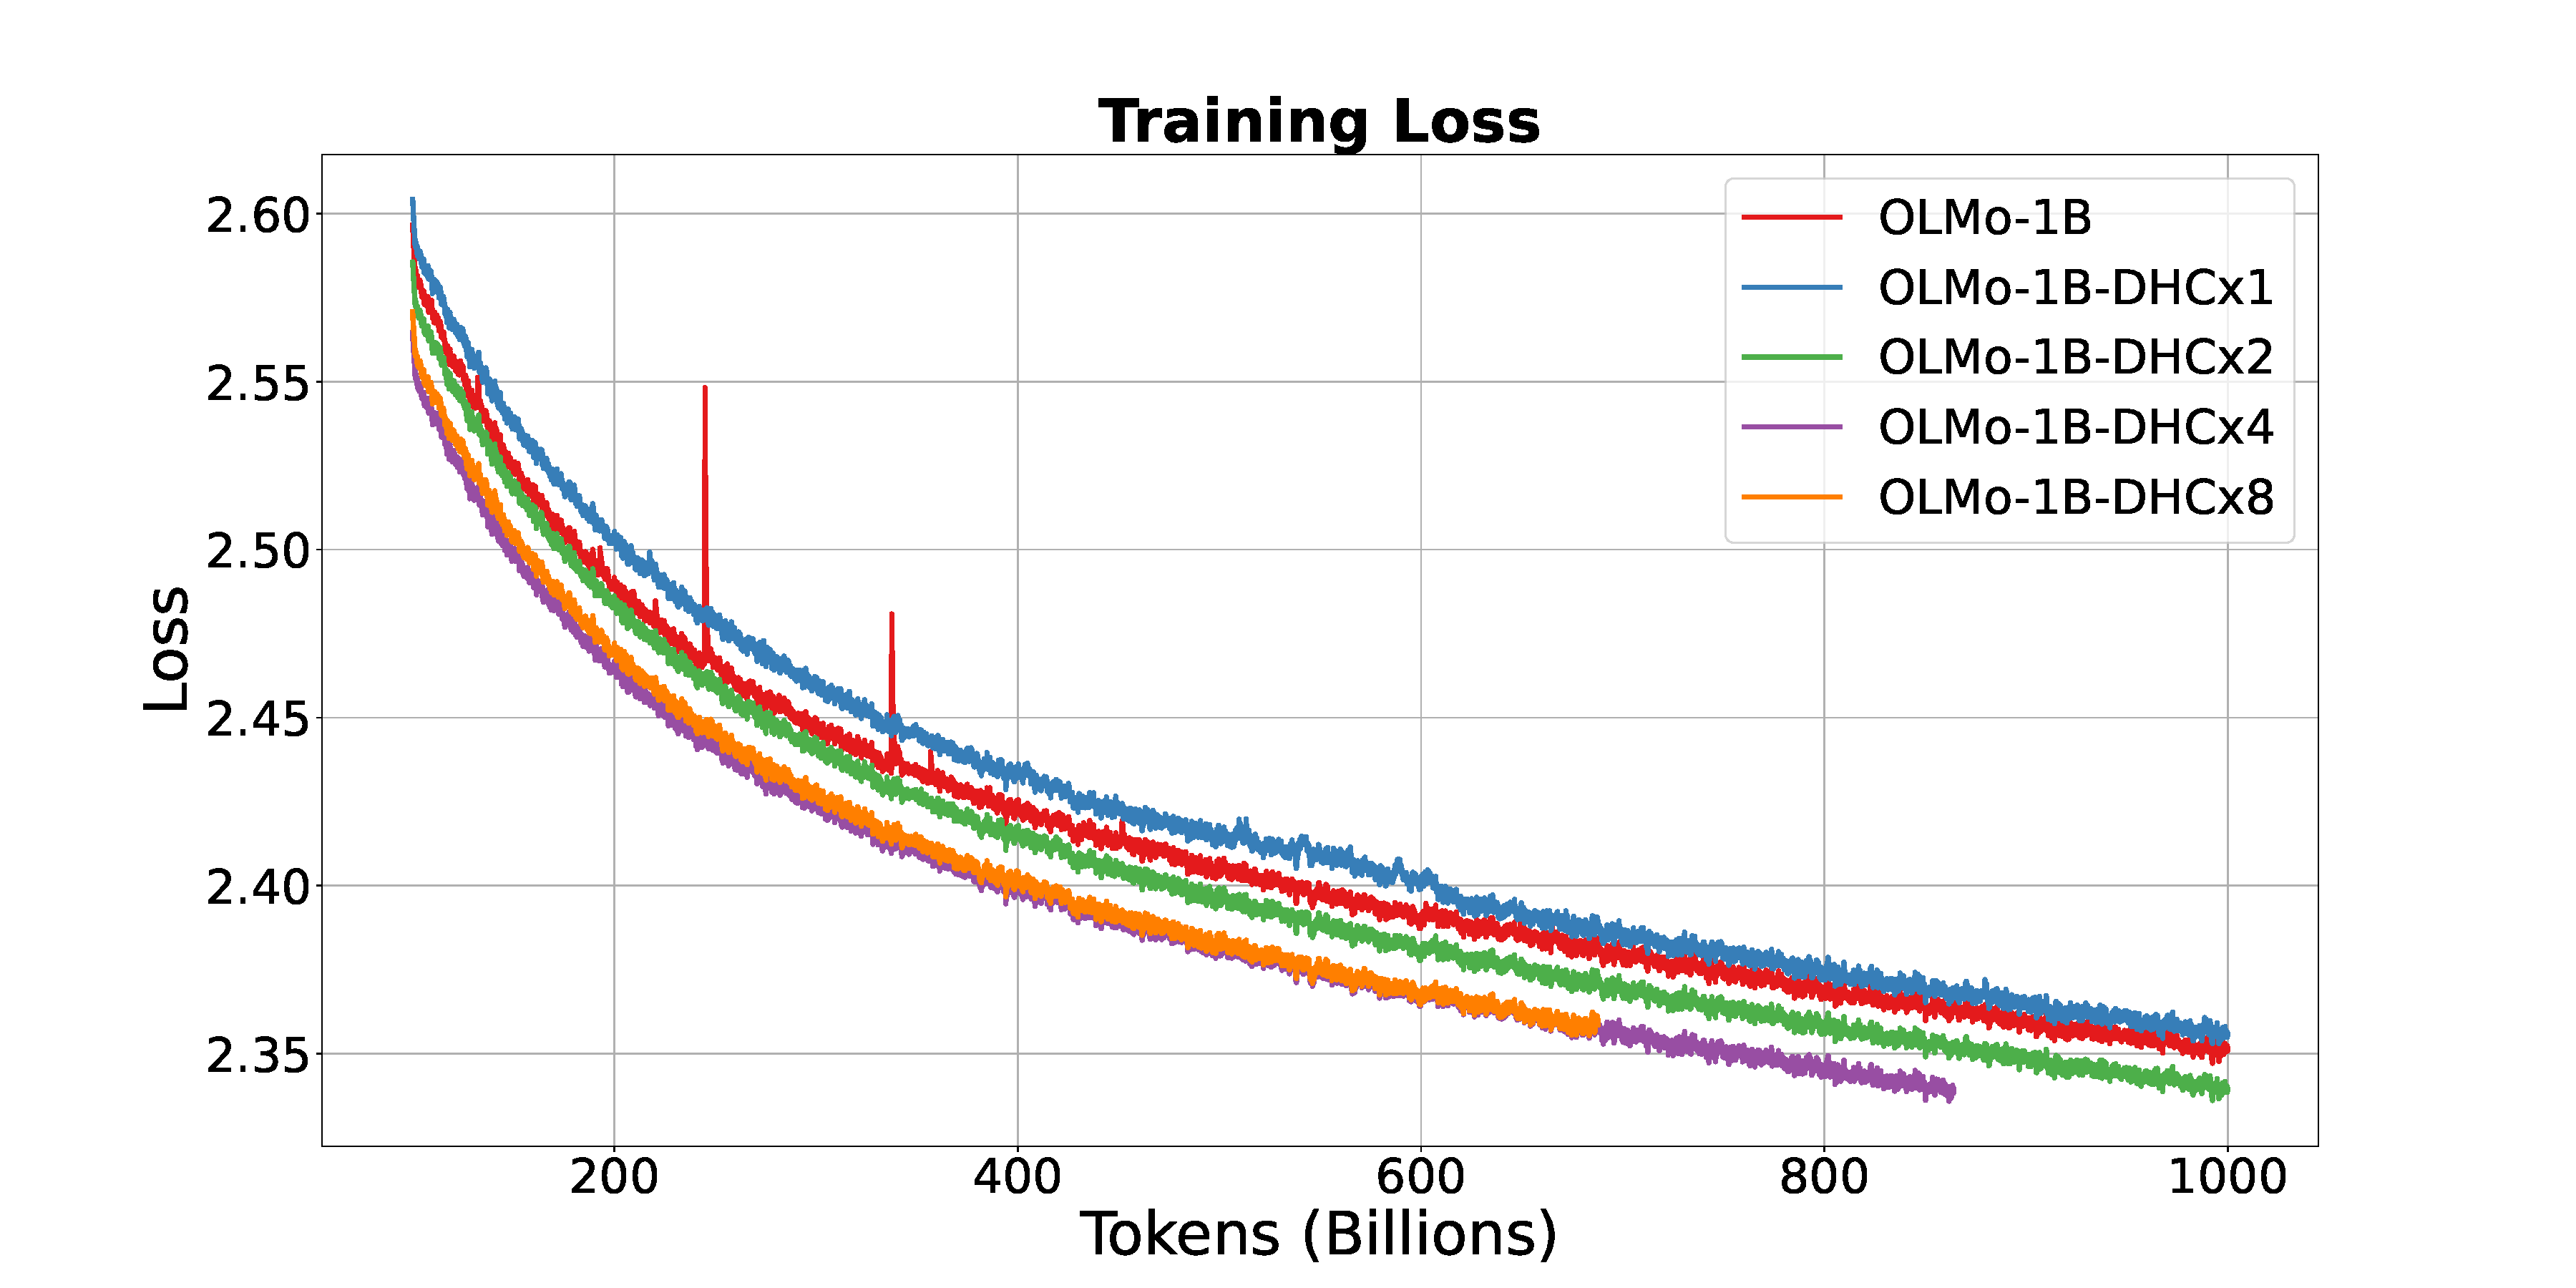
\includegraphics[width=1\textwidth]{fig/appendix_train_loss_olmo_1b_tanh_exp_099.pdf}
    \end{center}
  \caption{\newtext{Training loss curves of DHC with \texttt{tanh} over 500 billion tokens, smoothed using Exponential Moving Average (EMA) with a decay rate of 0.99.}}
    \label{fig:trans_with_hc}
\end{figure}

\begin{figure}[h]
    \begin{center}
    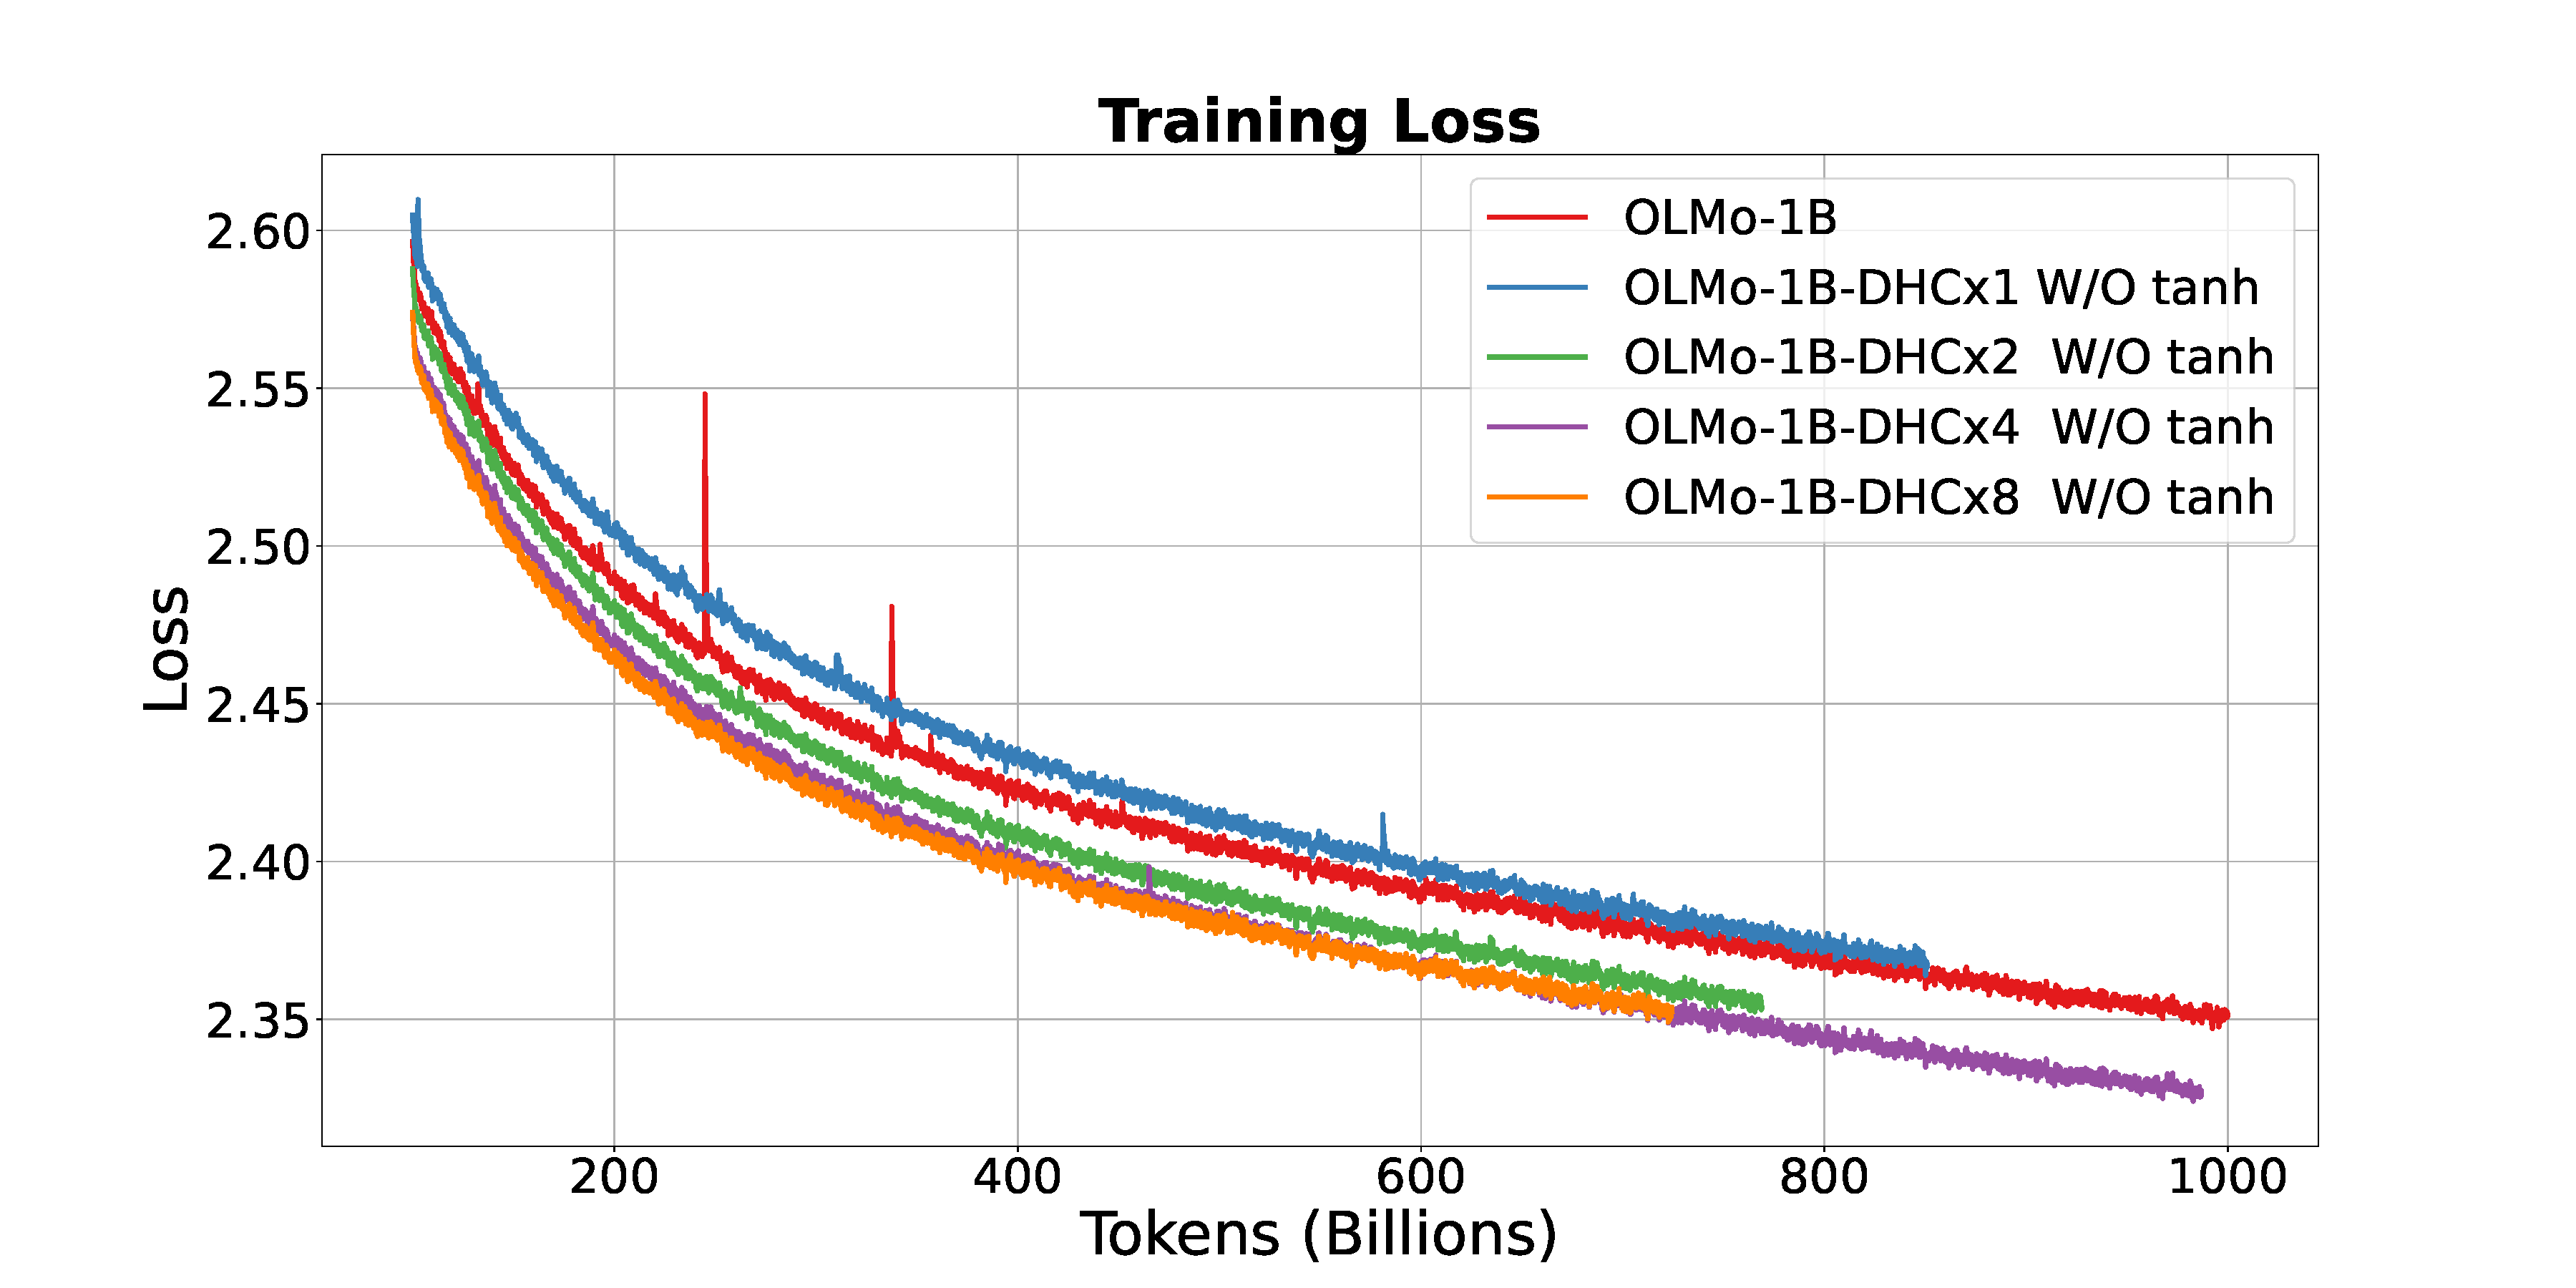
\includegraphics[width=1\textwidth]{fig/appendix_train_loss_olmo_1b_linear_exp_099.pdf}
    \end{center}
  \caption{\newtext{Training loss curves of DHC without \texttt{tanh} over 500 billion tokens, smoothed using Exponential Moving Average (EMA) with a decay rate of 0.99.}}
    \label{fig:trans_with_hc}
\end{figure}

\begin{table}[h]
\centering
\caption{Results on downstream benchmarks for 1B models.}
\small
\begin{tabular}{lcccccccr}
\toprule
\textbf{Method} & \textbf{arc\_easy} & \textbf{copa} & \textbf{hellaswag} & \textbf{openbook\_qa} & \textbf{piqa} & \textbf{sciq} & \textbf{winogrande} & \textbf{avg.} \\
\midrule
OLMo-1B & 56.8 & 76.0 & 56.1 & 33.8 & 74.4 & 85.1 & 55.6 & 62.5 \\
\midrule  
\multicolumn{9}{c}{ \cellcolor{gray!20} Scaling n in DHC W/O tanh} \\
\midrule
OLMo-1B-DHCx1 W/O tanh & 56.8 & 75.0 & 55.3 & 33.4 & 72.9 & 85.4 & 57.1 & 62.3 \\
OLMo-1B-DHCx2 W/O tanh & 63.0 & 74.0 & 57.1 & 34.6 & 73.5 & 86.0 & 58.2 & 63.8 \\
OLMo-1B-DHCx4 W/O tanh & 61.2 & 80.0 & 57.5 & 33.6 & 75.5 & 85.8 & 56.9 & 64.4 \\
OLMo-1B-DHCx8 W/O tanh & 61.1 & 75.0 & 57.6 & 35.4 & 73.8 & 85.2 & 58.5 & 63.8 \\
\midrule
\multicolumn{9}{c}{\cellcolor{gray!20} Scaling n in DHC} \\
\midrule
OLMo-1B-DHCx1 & 59.7 & 74.0 & 55.5 & 33.6 & 73.5 & 85.4 & 54.5 & 62.3 \\
OLMo-1B-DHCx2 & 59.7 & 73.0 & 56.7 & 34.0 & 74.7 & 85.2 & 57.9 & 63.0 \\
OLMo-1B-DHCx4 & 59.8 & 79.0 & 58.1 & 32.4 & 74.3 & 86.1 & 57.1 & 63.8 \\
OLMo-1B-DHCx8 & 56.8 & 75.0 & 58.0 & 34.4 & 73.8 & 84.2 & 57.3 & 62.8 \\
\midrule
\multicolumn{9}{c}{\cellcolor{gray!20} Scaling n in SHC} \\
\midrule
OLMo-1B-SHCx2 & 59.1 & 77.0 & 56.6 & 35.4 & 74.2 & 85.3 & 56.4 & 63.4 \\
OLMo-1B-SHCx4 & 59.3 & 77.0 & 56.7 & 34.0 & 74.3 & 86.6 & 57.1 & 63.6 \\
\midrule
\multicolumn{9}{c}{\cellcolor{gray!20} Non-trainable $\mathcal{WC}$} \\
\midrule
OLMo-1B-DHCx4 & 60.5 & 78.0 & 56.2 & 34.0 & 73.5 & 86.0 & 55.8 & 63.4 \\
OLMo-1B-DHCx4 W/O tanh & 59.1 & 72.0 & 56.8 & 35.0 & 73.3 & 86.0 & 55.5 & 62.5 \\
\midrule
\multicolumn{9}{c}{\cellcolor{gray!20} Non-trainable $\mathbf{B}$} \\
\midrule
OLMo-1B-DHCx4 & 59.5 & 77.0 & 57.9 & 33.8 & 73.3 & 85.6 & 56.6 & 63.4 \\
OLMo-1B-DHCx4 W/O tanh & 60.4 & 74.0 & 57.6 & 34.0 & 74.9 & 86.7 & 57.5 & 63.6 \\
\bottomrule
\end{tabular}
\label{tab:downstream_benchmarks}
\end{table}




\begin{table}[h]
\centering
\rotatebox{270}{
\begin{minipage}{\textheight}
\centering
\caption{Losses of V2 validation sets for 1B Model.}
\tiny
\begin{tabular}{lcccccccccccccr}
\toprule
\textbf{Method} & \textbf{4chan} & \textbf{c4\_100\_domains} & \textbf{c4\_en} & \textbf{gab} & \textbf{ice} & \textbf{m2d2\_s2orc} & \textbf{m2d2\_wiki} & \textbf{manosphere} & \textbf{mc4\_en} & \textbf{pile} & \textbf{ptb} & \textbf{twitterAAE} & \textbf{wikitext\_103} & \textbf{avg} \\
\midrule
OLMo-1B & 2.319 & 2.615 & 2.762 & 3.364 & 2.719 & 3.085 & 2.594 & 3.028 & 2.522 & 2.250 & 2.953 & 3.672 & 2.657 & 2.811 \\
\midrule
\multicolumn{15}{c}{\cellcolor{gray!20} Scaling n in DHC W/O tanh} \\
\midrule
OLMo-1B-DHCx1 W/O tanh & 2.320 & 2.626 & 2.773 & 3.379 & 2.725 & 3.102 & 2.609 & 3.036 & 2.531 & 2.264 & 2.948 & 3.703 & 2.672 & 2.822 \\
OLMo-1B-DHCx2 W/O tanh & 2.311 & 2.600 & 2.749 & 3.362 & 2.700 & 3.069 & 2.583 & 3.015 & 2.503 & 2.231 & 2.908 & 3.635 & 2.625 & 2.792 \\
OLMo-1B-DHCx4 W/O tanh & 2.295 & 2.591 & 2.735 & 3.344 & 2.686 & 3.056 & 2.562 & 3.005 & 2.492 & 2.221 & 2.898 & 3.632 & 2.610 & 2.779 \\
OLMo-1B-DHCx8 W/O tanh & 2.292 & 2.589 & 2.734 & 3.350 & 2.685 & 3.060 & 2.562 & 3.006 & 2.492 & 2.218 & 2.878 & 3.628 & 2.609 & 2.777 \\
\midrule
\multicolumn{15}{c}{\cellcolor{gray!20} Scaling n in DHC} \\
\midrule
OLMo-1B-DHCx1 & 2.323 & 2.625 & 2.775 & 3.376 & 2.728 & 3.090 & 2.606 & 3.037 & 2.533 & 2.262 & 2.961 & 3.652 & 2.678 & 2.819 \\
OLMo-1B-DHCx2 & 2.309 & 2.608 & 2.754 & 3.367 & 2.703 & 3.061 & 2.587 & 3.022 & 2.509 & 2.237 & 2.930 & 3.704 & 2.636 & 2.802 \\
OLMo-1B-DHCx4 & 2.290 & 2.591 & 2.738 & 3.354 & 2.683 & 3.064 & 2.564 & 3.005 & 2.492 & 2.218 & 2.890 & 3.641 & 2.611 & 2.781 \\
OLMo-1B-DHCx8 & 2.295 & 2.591 & 2.739 & 3.353 & 2.684 & 3.054 & 2.567 & 3.008 & 2.493 & 2.219 & 2.876 & 3.631 & 2.608 & 2.778 \\
\midrule
\multicolumn{15}{c}{\cellcolor{gray!20} Scaling n in SHC} \\
\midrule
OLMo-1B-SHCx2 & 2.307 & 2.610 & 2.757 & 3.360 & 2.703 & 3.063 & 2.587 & 3.023 & 2.511 & 2.238 & 2.933 & 3.643 & 2.643 & 2.799 \\
OLMo-1B-SHCx4 & 2.300 & 2.603 & 2.751 & 3.357 & 2.692 & 3.062 & 2.580 & 3.018 & 2.504 & 2.232 & 2.899 & 3.653 & 2.627 & 2.791 \\
\midrule
\multicolumn{15}{c}{\cellcolor{gray!20} Non-trainable WC} \\
\midrule
OLMo-1B-DHCx4 & 2.312 & 2.608 & 2.752 & 3.357 & 2.700 & 3.077 & 2.583 & 3.024 & 2.508 & 2.238 & 2.959 & 3.678 & 2.636 & 2.802 \\
OLMo-1B-DHCx4 W/O tanh & 2.308 & 2.609 & 2.755 & 3.357 & 2.710 & 3.100 & 2.585 & 3.025 & 2.510 & 2.240 & 2.945 & 3.663 & 2.644 & 2.804 \\
\midrule
\multicolumn{15}{c}{\cellcolor{gray!20} Non-trainable Beta} \\
\midrule
OLMo-1B-DHCx4 & 2.296 & 2.594 & 2.742 & 3.348 & 2.684 & 3.051 & 2.569 & 3.008 & 2.497 & 2.221 & 2.917 & 3.627 & 2.622 & 2.783 \\
OLMo-1B-DHCx4 W/O tanh & 2.295 & 2.592 & 2.739 & 3.347 & 2.689 & 3.066 & 2.567 & 3.005 & 2.496 & 2.222 & 2.887 & 3.638 & 2.606 & 2.781 \\
\bottomrule
\end{tabular}
\label{tab:v2_validation_set_loss}
\end{minipage}
}
\end{table}



\begin{table}[h]
\centering
\rotatebox{270}{
\begin{minipage}{\textheight}
\centering
\caption{Perplexities of V2 validation sets for 1B models.}
\tiny
\begin{tabular}{lcccccccccccccr}
\toprule
\textbf{Method} & \textbf{4chan} & \textbf{c4\_100\_domains} & \textbf{c4\_en} & \textbf{gab} & \textbf{ice} & \textbf{m2d2\_s2orc} & \textbf{m2d2\_wiki} & \textbf{manosphere} & \textbf{mc4\_en} & \textbf{pile} & \textbf{ptb} & \textbf{twitterAAE} & \textbf{wikitext\_103} & \textbf{avg} \\
\midrule
OLMo-1B & 10.167 & 13.666 & 15.829 & 28.901 & 15.166 & 21.860 & 13.377 & 20.651 & 12.453 & 9.488 & 19.161 & 39.328 & 14.251 & 18.023 \\
\midrule
\multicolumn{15}{c}{\cellcolor{gray!20} Scaling n in DHC W/O tanh} \\
\midrule
OLMo-1B-DHCx1 W/O tanh & 10.174 & 13.815 & 16.004 & 29.328 & 15.259 & 22.231 & 13.587 & 20.823 & 12.562 & 9.620 & 19.071 & 40.580 & 14.462 & 18.270 \\
OLMo-1B-DHCx2 W/O tanh & 9.920 & 13.340 & 15.412 & 28.340 & 14.676 & 21.243 & 12.965 & 20.181 & 12.079 & 9.219 & 18.129 & 37.768 & 13.594 & 17.451 \\
OLMo-1B-DHCx4 W/O tanh & 10.082 & 13.470 & 15.625 & 28.848 & 14.882 & 21.521 & 13.234 & 20.392 & 12.217 & 9.312 & 18.321 & 37.905 & 13.806 & 17.663 \\
OLMo-1B-DHCx8 W/O tanh & 9.897 & 13.313 & 15.387 & 28.488 & 14.658 & 21.337 & 12.960 & 20.200 & 12.084 & 9.185 & 17.782 & 37.650 & 13.592 & 17.425 \\
\midrule
\multicolumn{15}{c}{\cellcolor{gray!20} Scaling n in DHC} \\
\midrule
OLMo-1B-DHCx1 & 10.210 & 13.810 & 16.031 & 29.265 & 15.302 & 21.986 & 13.539 & 20.847 & 12.584 & 9.606 & 19.326 & 38.564 & 14.555 & 18.125 \\
OLMo-1B-DHCx2 & 10.061 & 13.568 & 15.710 & 29.002 & 14.925 & 21.349 & 13.284 & 20.524 & 12.294 & 9.362 & 18.727 & 40.592 & 13.957 & 17.950 \\
OLMo-1B-DHCx4 & 9.877 & 13.344 & 15.430 & 28.624 & 14.633 & 21.410 & 13.006 & 20.186 & 12.080 & 9.189 & 18.102 & 38.136 & 13.606 & 17.509 \\
OLMo-1B-DHCx8 & 9.922 & 13.346 & 15.467 & 28.591 & 14.640 & 21.198 & 13.025 & 20.240 & 12.097 & 9.196 & 17.749 & 37.743 & 13.570 & 17.445 \\
\midrule
\multicolumn{15}{c}{\cellcolor{gray!20} Scaling n in SHC} \\
\midrule
OLMo-1B-SHCx2 & 10.046 & 13.601 & 15.753 & 28.782 & 14.931 & 21.391 & 13.294 & 20.562 & 12.319 & 9.374 & 18.791 & 38.212 & 14.060 & 17.778 \\
OLMo-1B-SHCx4 & 9.977 & 13.507 & 15.655 & 28.691 & 14.766 & 21.372 & 13.194 & 20.457 & 12.234 & 9.315 & 18.149 & 38.569 & 13.836 & 17.671 \\
\midrule
\multicolumn{15}{c}{\cellcolor{gray!20} Non-trainable WC} \\
\midrule
OLMo-1B-DHCx4 & 10.054 & 13.587 & 15.721 & 28.689 & 15.023 & 22.186 & 13.263 & 20.594 & 12.310 & 9.390 & 19.016 & 38.959 & 14.070 & 17.912 \\
OLMo-1B-DHCx4 W/O tanh & 10.092 & 13.566 & 15.666 & 28.704 & 14.873 & 21.696 & 13.242 & 20.579 & 12.276 & 9.377 & 19.272 & 39.570 & 13.963 & 17.914 \\
\midrule
\multicolumn{15}{c}{\cellcolor{gray!20} Non-trainable Beta} \\
\midrule
OLMo-1B-DHCx4 & 9.927 & 13.354 & 15.475 & 28.417 & 14.722 & 21.454 & 13.021 & 20.185 & 12.135 & 9.228 & 17.932 & 38.005 & 13.553 & 17.493 \\
OLMo-1B-DHCx4 W/O tanh & 9.932 & 13.386 & 15.510 & 28.436 & 14.641 & 21.130 & 13.051 & 20.253 & 12.142 & 9.220 & 18.478 & 37.610 & 13.766 & 17.504 \\
\bottomrule
\end{tabular}
\label{tab:v2_validation_set_perplexity}
\end{minipage}
}
\end{table}


\begin{table}[h]
\centering
\rotatebox{270}{
\begin{minipage}{\textheight}
\centering
\caption{Losses of V3 validation sets  for 1B model.}
\tiny
\begin{tabular}{lcccccccccccr}
\toprule
\textbf{Method} & \textbf{c4\_en} & \textbf{dolma\_books} & \textbf{dolma\_common-crawl} & \textbf{dolma\_pes2o} & \textbf{dolma\_reddit} & \textbf{dolma\_stack} & \textbf{dolma\_wiki} & \textbf{ice} & \textbf{m2d2\_s2orc} & \textbf{pile} & \textbf{wikitext\_103} & \textbf{avg} \\
\midrule
OLMo-1B & 2.702 & 2.906 & 2.722 & 2.333 & 2.980 & 1.041 & 2.487 & 2.715 & 3.199 & 2.232 & 2.663 & 2.544 \\
\midrule
\multicolumn{13}{c}{\cellcolor{gray!20} Scaling n in DHC W/O tanh} \\
\midrule
OLMo-1B-DHCx1 W/O tanh & 2.712 & 2.928 & 2.732 & 2.349 & 2.991 & 1.045 & 2.499 & 2.721 & 3.219 & 2.246 & 2.677 & 2.556 \\
OLMo-1B-DHCx2 W/O tanh & 2.676 & 2.880 & 2.698 & 2.306 & 2.961 & 1.024 & 2.456 & 2.682 & 3.174 & 2.204 & 2.617 & 2.516 \\
OLMo-1B-DHCx4 W/O tanh & 2.689 & 2.890 & 2.706 & 2.317 & 2.969 & 1.030 & 2.471 & 2.697 & 3.200 & 2.213 & 2.633 & 2.529 \\
OLMo-1B-DHCx8 W/O tanh & 2.674 & 2.876 & 2.695 & 2.303 & 2.960 & 1.022 & 2.454 & 2.680 & 3.176 & 2.200 & 2.616 & 2.514 \\
\midrule
\multicolumn{13}{c}{\cellcolor{gray!20} Scaling n in DHC} \\
\midrule
OLMo-1B-DHCx1 & 2.714 & 2.927 & 2.732 & 2.346 & 2.991 & 1.045 & 2.499 & 2.723 & 3.211 & 2.245 & 2.683 & 2.556 \\
OLMo-1B-DHCx2 & 2.694 & 2.901 & 2.712 & 2.321 & 2.976 & 1.032 & 2.478 & 2.699 & 3.202 & 2.218 & 2.642 & 2.534 \\
OLMo-1B-DHCx4 & 2.675 & 2.876 & 2.697 & 2.301 & 2.962 & 1.021 & 2.455 & 2.679 & 3.176 & 2.200 & 2.617 & 2.515 \\
OLMo-1B-DHCx8 & 2.677 & 2.880 & 2.701 & 2.304 & 2.964 & 1.022 & 2.456 & 2.680 & 3.177 & 2.201 & 2.614 & 2.516 \\
\midrule
\multicolumn{13}{c}{\cellcolor{gray!20} Scaling n in SHC} \\
\midrule
OLMo-1B-SHCx2 & 2.698 & 2.907 & 2.718 & 2.325 & 2.980 & 1.032 & 2.479 & 2.700 & 3.198 & 2.221 & 2.650 & 2.537 \\
OLMo-1B-SHCx4 & 2.689 & 2.892 & 2.711 & 2.315 & 2.973 & 1.028 & 2.472 & 2.688 & 3.195 & 2.214 & 2.633 & 2.528 \\
\midrule
\multicolumn{13}{c}{\cellcolor{gray!20} Non-trainable WC} \\
\midrule
OLMo-1B-DHCx4 & 2.695 & 2.903 & 2.716 & 2.324 & 2.978 & 1.035 & 2.477 & 2.705 & 3.201 & 2.221 & 2.649 & 2.537 \\
OLMo-1B-DHCx4 W/O tanh & 2.692 & 2.899 & 2.714 & 2.321 & 2.976 & 1.032 & 2.474 & 2.695 & 3.189 & 2.219 & 2.641 & 2.532 \\
\midrule
\multicolumn{13}{c}{\cellcolor{gray!20} Non-trainable Beta} \\
\midrule
OLMo-1B-DHCx4 & 2.679 & 2.880 & 2.697 & 2.306 & 2.961 & 1.025 & 2.458 & 2.684 & 3.188 & 2.204 & 2.612 & 2.518 \\
OLMo-1B-DHCx4 W/O tanh & 2.681 & 2.886 & 2.702 & 2.306 & 2.966 & 1.024 & 2.462 & 2.680 & 3.183 & 2.204 & 2.628 & 2.520 \\
\bottomrule
\end{tabular}
\label{tab:v3_validation_set_loss}
\end{minipage}
}
\end{table}


\begin{table}[h]
\centering
\rotatebox{270}{
\begin{minipage}{\textheight}
\centering
\caption{Perplexities of V3 validation sets for 1B models.}
\tiny
\begin{tabular}{lcccccccccccr}
\toprule
\textbf{Method} & \textbf{c4\_en} & \textbf{dolma\_books} & \textbf{dolma\_common-crawl} & \textbf{dolma\_pes2o} & \textbf{dolma\_reddit} & \textbf{dolma\_stack} & \textbf{dolma\_wiki} & \textbf{ice} & \textbf{m2d2\_s2orc} & \textbf{pile} & \textbf{wikitext\_103} & \textbf{avg} \\
\midrule
OLMo-1B & 14.908 & 18.289 & 15.216 & 10.305 & 19.686 & 2.832 & 12.026 & 15.098 & 24.503 & 9.319 & 14.334 & 14.229 \\
\midrule
\multicolumn{13}{c}{\cellcolor{gray!20} Scaling n in DHC W/O tanh} \\
\midrule
OLMo-1B-DHCx1 W/O tanh & 15.064 & 18.699 & 15.356 & 10.473 & 19.909 & 2.843 & 12.167 & 15.191 & 25.013 & 9.451 & 14.540 & 14.428 \\
OLMo-1B-DHCx2 W/O tanh & 14.531 & 17.817 & 14.857 & 10.038 & 19.323 & 2.783 & 11.662 & 14.608 & 23.906 & 9.061 & 13.694 & 13.844 \\
OLMo-1B-DHCx4 W/O tanh & 14.711 & 17.996 & 14.975 & 10.146 & 19.479 & 2.800 & 11.830 & 14.839 & 24.524 & 9.146 & 13.917 & 14.033 \\
OLMo-1B-DHCx8 W/O tanh & 14.494 & 17.749 & 14.813 & 10.000 & 19.306 & 2.779 & 11.630 & 14.587 & 23.948 & 9.021 & 13.684 & 13.819 \\
\midrule
\multicolumn{13}{c}{\cellcolor{gray!20} Scaling n in DHC} \\
\midrule
OLMo-1B-DHCx1 & 15.093 & 18.675 & 15.360 & 10.442 & 19.909 & 2.845 & 12.174 & 15.225 & 24.810 & 9.436 & 14.632 & 14.418 \\
OLMo-1B-DHCx2 & 14.794 & 18.190 & 15.061 & 10.191 & 19.612 & 2.806 & 11.915 & 14.870 & 24.589 & 9.187 & 14.043 & 14.114 \\
OLMo-1B-DHCx4 & 14.514 & 17.743 & 14.829 & 9.989 & 19.343 & 2.776 & 11.650 & 14.573 & 23.948 & 9.028 & 13.689 & 13.826 \\
OLMo-1B-DHCx8 & 14.546 & 17.807 & 14.889 & 10.011 & 19.366 & 2.779 & 11.653 & 14.579 & 23.964 & 9.030 & 13.653 & 13.843 \\
\midrule
\multicolumn{13}{c}{\cellcolor{gray!20} Scaling n in SHC} \\
\midrule
OLMo-1B-SHCx2 & 14.854 & 18.293 & 15.150 & 10.230 & 19.689 & 2.807 & 11.934 & 14.876 & 24.478 & 9.214 & 14.150 & 14.152 \\
OLMo-1B-SHCx4 & 14.717 & 18.028 & 15.049 & 10.121 & 19.550 & 2.796 & 11.846 & 14.699 & 24.407 & 9.155 & 13.912 & 14.025 \\
\midrule
\multicolumn{13}{c}{\cellcolor{gray!20} Non-trainable WC} \\
\midrule
OLMo-1B-DHCx4 & 14.810 & 18.224 & 15.120 & 10.215 & 19.650 & 2.816 & 11.902 & 14.954 & 24.552 & 9.220 & 14.135 & 14.145 \\
OLMo-1B-DHCx4 W/O tanh & 14.756 & 18.160 & 15.095 & 10.191 & 19.613 & 2.806 & 11.868 & 14.807 & 24.273 & 9.203 & 14.021 & 14.072 \\
\midrule
\multicolumn{13}{c}{\cellcolor{gray!20} Non-trainable Beta} \\
\midrule
OLMo-1B-DHCx4 & 14.574 & 17.820 & 14.840 & 10.038 & 19.320 & 2.787 & 11.677 & 14.647 & 24.233 & 9.059 & 13.621 & 13.874 \\
OLMo-1B-DHCx4 W/O tanh & 14.593 & 17.926 & 14.904 & 10.032 & 19.405 & 2.785 & 11.724 & 14.588 & 24.108 & 9.060 & 13.839 & 13.906 \\
\bottomrule
\end{tabular}
\label{tab:v3_validation_set_perplexity}
\end{minipage}
}
\end{table}